% \documentclass[8pt]{beamer}

% \usetheme{metropolis}

% \usepackage[export]{adjustbox}
% \usepackage{amsmath}
% \usepackage{bbm}
% \usepackage{emoji}
% \usepackage{pgfplots}
% \usepackage{hyperref}
% \usepackage{listings}
% \usepackage{tcolorbox}
% \usepackage{xcolor}

% \usepgfplotslibrary{groupplots}

% \usetikzlibrary{arrows.meta}
% \usetikzlibrary{calc}
\documentclass[8pt]{beamer}

\usetheme{metropolis}

\usepackage[export]{adjustbox}
\usepackage{array}
\usepackage{bbm}
\usepackage{emoji}
\usepackage{etoolbox}
\usepackage{graphicx}
\usepackage{hyperref}
\usepackage{listings}
\usepackage{pgfplots}
\usepackage{tikz}
\usepackage{xcolor}

\usepgfplotslibrary{fillbetween}
\usepgfplotslibrary{groupplots}

\usetikzlibrary{arrows.meta}
\usetikzlibrary{calc}
\usetikzlibrary{patterns}

\hypersetup{
    colorlinks=true,
    linkcolor=white,
    urlcolor=blue!80
}

\definecolor{uiored}{HTML}{DD0000}
\definecolor{uiolightred}{HTML}{FB6666}
\definecolor{uioredtone}{HTML}{FEE0E0}
\definecolor{uioblue}{HTML}{3E31D6}
\definecolor{uiolightblue}{HTML}{86A4F7}
\definecolor{uioblueone}{HTML}{E6ECFF}
\definecolor{uiogreen}{HTML}{2EC483}
\definecolor{uiolightgreen}{HTML}{6CE1AB}
\definecolor{uiogreentone}{HTML}{CEFFDF}
\definecolor{uioorange}{HTML}{FEA11B}
\definecolor{uiolightorange}{HTML}{FDCB87}
\definecolor{uioorangetone}{HTML}{FFE8D4}
\definecolor{uioyellow}{HTML}{FFFEA7}
\definecolor{uiogray}{HTML}{B2B3B7}

\colorlet{mainbackground}{uiored}

\setbeamercolor{frametitle}{bg=mainbackground, fg=white}
\setbeamercolor{title separator}{fg=mainbackground}
\setbeamercolor{progress bar in section page}{fg=white, bg=uiogray}

\def\logowidth{4cm}

\makeatletter
\setbeamertemplate{section page}
{
  \begingroup

    \vspace{4.3cm}
    {\usebeamercolor[fg]{section title}\usebeamerfont{section title}\insertsectionhead}\\[-1ex]
    {\centering\color{white}\rule{\linewidth}{1pt}\par} % the horizontal line

    \vspace*{3.1cm}
    \begin{center}
        
\includegraphics[width=\logowidth,valign=c]{data/uio_logo_full_white.png} % Adjust width and path to your logo as needed
    \end{center}

  \endgroup
}
\makeatother

\AtBeginSection{
  {
    \setbeamercolor{background canvas}{bg=uiored}
    \setbeamercolor{section title}{fg=white}
    \frame[plain,c,noframenumbering]{\sectionpage}
    \setbeamercolor{background canvas}{bg=black!2}
  }
}



\setbeamertemplate{footline}{
    \ifnum\insertframenumber=1
        % Title page, no footer
    \else
        \begin{tikzpicture}[remember picture,overlay]
            \fill[mainbackground] (current page.south west) rectangle ([yshift=0.45cm]current page.south east); % Draw filled rectangle

            % Logo
            \node[anchor=west, yshift=0.225cm] at (current page.south west) {
\includegraphics[height=1.2cm]{data/uio_logo_white.png}};

            % Title and subtitle
            \node[align=center, yshift=0.225cm] at (current page.south) {\textcolor{white}{\textbf{\inserttitle}}\\[0.05cm]\textcolor{white}{\insertsubtitle}};

            % Page number
            \node[anchor=east, yshift=0.225cm, xshift=-0.2cm, align=right] at (current page.south east) {\textcolor{white}{\insertframenumber/\inserttotalframenumber}};
        \end{tikzpicture}
    \fi
}

\lstdefinestyle{Core}{
    identifierstyle=\color[RGB]{0, 0, 0},
    stringstyle=\color[RGB]{205, 49, 49},
    showstringspaces=false,
    breaklines,
    xleftmargin=3pt,
    xrightmargin=3pt,
    framesep=3pt,
    aboveskip=-1.5pt,
    belowskip=-0.5pt,
    showlines=true,
}

\lstdefinestyle{RInput}{
    style=Core,
    language=R,
    keywordstyle=\color[RGB]{17, 115, 187},
    commentstyle=\color[RGB]{0, 128, 0},
    identifierstyle=\color[RGB]{0, 0, 0},
    stringstyle=\color[RGB]{205, 49, 49},
    backgroundcolor=\color[RGB]{255, 255, 255},
    frame=single,
    rulecolor=\color[RGB]{0, 0, 0},
}

\lstdefinestyle{PythonInput}{
    style=Core,
    language=Python,
    keywordstyle=\color[RGB]{26, 13, 171},
    commentstyle=\color[RGB]{0, 128, 0},
    backgroundcolor=\color[RGB]{245, 245, 245},
    rulecolor=\color[RGB]{192, 192, 192},
    frame=tblr,
}

\lstdefinestyle{ROutput}{
    style=Core,
    language=R,
    backgroundcolor=\color[RGB]{255, 255, 255},
    commentstyle=\color[HTML]{009900},
    stringstyle=\color[HTML]{0000FF},
    keywordstyle=\color[HTML]{000000},
    numberstyle=\tiny\color[HTML]{000000},
    breakatwhitespace=true,
    frame=single,
    rulecolor=\color{black},
}

\lstdefinestyle{PythonOutput}{
    backgroundcolor=\color[RGB]{255, 255, 255},
    rulecolor=\color[RGB]{192, 192, 192},
    frame=single,
    numbers=none,
    showstringspaces=false,
    breakatwhitespace=true,
    keywordstyle=\color[RGB]{255, 0, 0},
    morekeywords={AttributeError}
}

\newcommand{\PythonInputNode}[6]{%
    \node[
        minimum width=#4,
        text width=#4,
        align=left,
        inner sep=0pt,
        outer sep=0pt,
        anchor=north west,
        label={[blue,
                anchor=north east,
                font=\ttfamily\fontsize{\the\numexpr#5-1\relax}{#5}\selectfont,
                inner sep=0pt,
                outer sep=0pt,
                xshift=-3pt,
                yshift=-3pt
                ]north west:In{[}#1{]}:},
    ] (#3) at #2 {
    \begin{lstlisting}[
        style=PythonInput,
        linewidth=#4,
        basicstyle=\ttfamily\fontsize{\the\numexpr#5-1\relax}{#5}\selectfont,
        numberstyle=\fontsize{\the\numexpr#5-1\relax}{#5}\selectfont\color[RGB]{128, 128, 128},
    ]^^J
        #6
    \end{lstlisting}
    };
}

\newcommand{\PythonOutputNode}[6]{%
    \node[
        minimum width=#4,
        text width=#4,
        align=left,
        inner sep=0pt,
        outer sep=0pt,
        anchor=north west,
        label={[red,
                anchor=north east,
                font=\ttfamily\fontsize{\the\numexpr#5-1\relax}{#5}\selectfont,
                inner sep=0pt,
                outer sep=0pt,
                xshift=-6pt,
                yshift=-11pt
                ]north west:Out{[}#1{]}:}
    ] (pythonoutput) (#3) at #2 {
        \begin{lstlisting}[
            style=PythonOutput,
            basicstyle=\ttfamily\fontsize{\the\numexpr#5-1\relax}{#5}\selectfont,
            numberstyle=\fontsize{\the\numexpr#5-1\relax}{#5}\selectfont\color[RGB]{128, 128, 128},
        ]^^J
            #6
        \end{lstlisting}
    };
}

\newcommand{\RInputNode}[5]{
    \node[
        minimum width=#3,
        text width=#3,
        align=left,
        inner sep=0pt,
        outer sep=0pt,
        draw=black,
        anchor=north west
    ] (#2) at #1 {
        \begin{lstlisting}[
            style=RInput,
            linewidth=\textwidth,
            basicstyle=\ttfamily\fontsize{\the\numexpr#4-1\relax}{#4}\selectfont,
            numberstyle=\fontsize{\the\numexpr#4-1\relax}{#4}\selectfont\color[RGB]{128, 128, 128},
        ]^^J
            #5
        \end{lstlisting}
    };
}

\title{PSY9511: Seminar 3}
\subtitle{Regularization and variable selection}
\author{Esten H. Leonardsen}
\date{11.09.24}

\begin{document}
	\begin{frame}
	 	\maketitle
	\end{frame}

    \begin{frame}{Outline}
        \centering
        \vfill
        \begin{enumerate}
            \item Assignment 1
            \item Assignment 2
            \item Regularization
            \begin{itemize}
                \item Variable selection
                \item Shrinkage (+ live coding \emoji{partying-face})
            \end{itemize}
        \end{enumerate}
        \vfill
    \end{frame}

    \section{Assignment 1}

    \begin{frame}[t]{Assignment 1: Coding}
        \vspace{2cm}
        \begin{itemize}
            \item Create a vector of 100 standard normally distributed numbers and visualize them with a histogram.
            \item Show rows 5, 8, 9, and 10 of the Auto dataset.
            \item Show the last three columns of the Auto dataset.
            \item Show all cars with five cylinders in the Auto dataset.
        \end{itemize}

        \only<2>{
            \vspace{0.5cm}
            \url{http://localhost:8889/notebooks/notebooks\%2FAssignment\%201.ipynb}
        }
    \end{frame}

    \newcommand{\flexplot}[1]{
        \begin{tikzpicture}
            \begin{axis}[
                height=4cm,
                width=4cm,
                xmajorticks=false,
                ymajorticks=false,
                xmin=0,
                xmax=1,
                ymin=0,
                ymax=1
            ]
                \addplot[
                    only marks,
                    mark=*,
                    color=blue,
                    opacity=0.1
                ] table [
                    col sep=comma,
                    y=y,
                    x=X
                ] {data/flexibility.csv};

                \ifnum#1<7
                    \ifnum#1=1
                        \def\col{simple}
                    \fi
                    \ifnum#1=2
                        \def\col{medium}
                    \fi
                    \ifnum#1=3
                        \def\col{complex}
                    \fi
                    \ifnum#1=4
                        \def\col{k1}
                    \fi
                    \ifnum#1=5
                        \def\col{k30}
                    \fi
                    \ifnum#1=6
                        \def\col{k100}
                    \fi

                    \addplot[
                        very thick,
                        red
                    ] table [
                        col sep=comma,
                        y=\col,
                        x=X
                    ] {data/flexibility.csv};
                \fi
                \ifnum#1=7
                    \addplot[
                        very thick,
                        orange
                    ] table [
                        col sep=comma,
                        y=k100,
                        x=X
                    ] {data/flexibility.csv};
                \fi
                \ifnum#1=8
                    \addplot[
                        very thick,
                        red
                    ] table [
                        col sep=comma,
                        y=k30,
                        x=X
                    ] {data/flexibility.csv};
                    \addplot[
                        very thick,
                        orange
                    ] table [
                        col sep=comma,
                        y=approx,
                        x=X
                    ] {data/flexibility.csv};
                \fi
            \end{axis}
        \end{tikzpicture}
    }

    \newsavebox{\flexsimple}
    \sbox{\flexsimple}{\flexplot{1}}

    \newsavebox{\flexmedium}
    \sbox{\flexmedium}{\flexplot{2}}

    \newsavebox{\flexcomplex}
    \sbox{\flexcomplex}{\flexplot{3}}

    \newsavebox{\flexkone}
    \sbox{\flexkone}{\flexplot{4}}
    \newsavebox{\flexkthirty}
    \sbox{\flexkthirty}{\flexplot{5}}
    \newsavebox{\flexkall}
    \sbox{\flexkall}{\flexplot{6}}
    \newsavebox{\flexapproxall}
    \sbox{\flexapproxall}{\flexplot{7}}
    \newsavebox{\flexapprox}
    \sbox{\flexapprox}{\flexplot{8}}

    \newcommand{\biasvariance}[1]{
        \begin{tikzpicture}
            \begin{axis}[
                xmin=-1,
                xmax=1,
                ymin=-1,
                ymax=1,
                height=4cm,
                width=4cm,
                axis line style={draw=none},
                xmajorticks=false,
                ymajorticks=false
            ]
                \node[circle, minimum size=2.4cm, draw=black, fill=blue!60] at (axis cs: 0, 0) {};
                \node[circle, minimum size=1.9cm, draw=none, fill=white] at (axis cs: 0, 0) {};
                \node[circle, minimum size=1.4cm, draw=none, fill=blue!60] at (axis cs: 0, 0) {};
                \node[circle, minimum size=0.9cm, draw=none, fill=white] at (axis cs: 0, 0) {};
                \node[circle, minimum size=0.4cm, draw=none, fill=red] at (axis cs: 0, 0) {};

                \ifnum#1>1
                    \ifnum#1=2
                        \def\xcol{X1}
                        \def\ycol{y1}
                    \fi
                    \ifnum#1=3
                        \def\xcol{X2}
                        \def\ycol{y2}
                    \fi
                    \ifnum#1=4
                        \def\xcol{X3}
                        \def\ycol{y3}
                    \fi
                    \ifnum#1=5
                        \def\xcol{X4}
                        \def\ycol{y4}
                    \fi

                    \addplot[
                        only marks
                    ] table [
                        col sep=comma,
                        x=\xcol,
                        y=\ycol
                    ] {data/bias-variance.csv};
                \fi
            \end{axis}

        \end{tikzpicture}
    }

    \newsavebox{\dart}
    \sbox{\dart}{\biasvariance{1}}
    \newsavebox{\lowlow}
    \sbox{\lowlow}{\biasvariance{2}}
    \newsavebox{\lowhigh}
    \sbox{\lowhigh}{\biasvariance{3}}
    \newsavebox{\highlow}
    \sbox{\highlow}{\biasvariance{4}}
    \newsavebox{\highhigh}
    \sbox{\highhigh}{\biasvariance{5}}

    \newcommand{\functionbox}[1]{
        \begin{tikzpicture}
            \begin{axis}[
                height=4cm,
                width=4cm,
                xmajorticks=false,
                ymajorticks=false,
                xmin=0,
                xmax=10,
                ymin=0,
                ymax=10
            ]

                \ifnum#1<4
                    \ifnum#1<3
                        \addplot[
                            only marks,
                            mark=*,
                            color=blue,
                            opacity=0.25
                        ] table [
                            col sep=comma,
                            y=noisy_periodic,
                            x=X
                        ] {data/functions.csv};
                    \fi
                    \ifnum#1=3
                        \addplot[
                            only marks,
                            mark=*,
                            color=teal,
                            opacity=0.25
                        ] table [
                            col sep=comma,
                            y=noisy_periodic2,
                            x=X
                        ] {data/functions.csv};
                    \fi

                    \addplot[
                        very thick,
                        blue
                    ] table [
                        col sep=comma,
                        x=X,
                        y=periodic
                    ] {data/functions.csv};

                    \ifnum#1>1
                        \addplot[
                            very thick,
                            orange
                        ] coordinates {
                            (0, 5)
                            (10, 5)
                        };
                    \fi
                \fi
                \ifnum#1>3
                    \ifnum#1<6
                        \addplot[
                            only marks,
                            mark=*,
                            color=blue,
                            opacity=0.25
                        ] table [
                            col sep=comma,
                            y=noisy,
                            x=X
                        ] {data/functions.csv};
                    \fi
                    \ifnum#1=6
                        \addplot[
                            only marks,
                            mark=*,
                            color=teal,
                            opacity=0.25
                        ] table [
                            col sep=comma,
                            y=noisy2,
                            x=X
                        ] {data/functions.csv};
                    \fi

                    \addplot[
                        very thick,
                        blue
                    ] table [
                        col sep=comma,
                        x=X,
                        y=X
                    ] {data/functions.csv};

                    \ifnum#1>4
                        \addplot[
                            very thick,
                            orange
                        ] table [
                            col sep=comma,
                            x=X,
                            y=noisy
                        ] {data/functions.csv};
                    \fi
                \fi
            \end{axis}
        \end{tikzpicture}
    }

    \newsavebox{\periodic}
    \sbox{\periodic}{\functionbox{1}}
    \newsavebox{\periodicfunction}
    \sbox{\periodicfunction}{\functionbox{2}}
    \newsavebox{\linear}
    \sbox{\linear}{\functionbox{4}}
    \newsavebox{\linearfunction}
    \sbox{\linearfunction}{\functionbox{5}}
    \newsavebox{\periodictest}
    \sbox{\periodictest}{\functionbox{3}}
    \newsavebox{\lineartest}
    \sbox{\lineartest}{\functionbox{6}}

    \begin{frame}{Assignment 2: Bias-variance trade-off}
        \only<1-9>{
            \begin{tikzpicture}
                \node[] at (-5.25, -3) {};
                \node[] at (5.25, 3) {};

                \only<2-6>{
                    \draw[-stealth] (-4, -1) -- (4, -1);
                }
                \only<2-3>{
                    \node[] at (0, -1.5) {Flexibility};
                }
                \only<3>{
                    \node[] at (-3, 1) {\usebox{\flexsimple}};
                    \node[] at (0, 1) {\usebox{\flexmedium}};
                    \node[] at (3, 1) {\usebox{\flexcomplex}};
                }
                \only<4-6>{
                    \node[] (kone) at (3, 1) {\usebox{\flexkone}};

                    \node[] at (0, -1.5) {Number of neighbours};
                    \draw[] (-3, -0.95) -- (-3, -1.05);
                    \node[anchor=north, inner sep=5pt] at (3, -1) {1};
                    \draw[] (3, -0.95) -- (3, -1.05);
                    \node[anchor=north, inner sep=5pt] at (-3, -1) {K};
                }
                \only<4>{
                    \node[] (kall) at (-3, 1) {\usebox{\flexkall}};
                }
                \only<4-5>{
                    \node[] (kthirty) at (0, 1) {\usebox{\flexkthirty}};
                }
                \only<5-9>{
                    \node[anchor=south,font=\tiny,orange, text depth=0] (formulak) at ($ (kall.south) - (0, 0.25) $) {$f(x)=0.39$};
                }
                \only<5-6>{
                    \node[] (kall) at (-3, 1) {\usebox{\flexapproxall}};
                }
                \only<6-9>{
                    \node[anchor=south,font=\tiny,orange, text depth=0] (formulaapprox) at ($ (kthirty.south) - (0, 0.25) $) {$f(x)=-3.57x^4+5.38x^3-1.22x^2+0.19x+0.03$};
                }
                \only<6>{
                    \node[] (kapprox) at (0, 1) {\usebox{\flexapprox}};
                }
                \only<8-9>{
                    \node[] (p11) at ($ (formulak.south) + (0.3, -0.3) $) {1};
                    \draw[-stealth] (p11.north) -- ($ (p11.north) + (0, 0.17) $);
                }\only<9>{
                    \node[] (p21) at ($ (formulaapprox.south) - (1.17, 0.3) $) {1};
                    \draw[-stealth] (p21.north) -- ($ (p21.north) + (0, 0.17) $);
                    \node[] (p22) at ($ (formulaapprox.south) - (0.32, 0.3) $) {2};
                    \draw[-stealth] (p22.north) -- ($ (p22.north) + (0, 0.17) $);
                    \node[] (p23) at ($ (formulaapprox.south) - (-0.44, 0.3) $) {3};
                    \draw[-stealth] (p23.north) -- ($ (p23.north) + (0, 0.17) $);
                    \node[] (p24) at ($ (formulaapprox.south) - (-1.26, 0.3) $) {4};
                    \draw[-stealth] (p24.north) -- ($ (p24.north) + (0, 0.17) $);
                    \node[] (p25) at ($ (formulaapprox.south) - (-1.95, 0.3) $) {5};
                    \draw[-stealth] (p25.north) -- ($ (p25.north) + (0, 0.17) $);
                }
            \end{tikzpicture}
        }
        \only<10>{
            Model flexibility: Denotes the complexity of the approximated function $\hat{y}=\hat{f}(x)$.
            \begin{itemize}
                \item Informally: Wigglyness of the line
                \item Formally: Number of parameters in the function (degrees of freedom)
            \end{itemize}
        }
        \only<11-15>{
            \begin{tikzpicture}
                \node[draw=black] at (-5.25, -3) {};
                \node[draw=black] at (5.25, 3) {};

                \only<11>{
                    \node[] at (-1.5, 1.25) {
                        \usebox{\dart}
                    };
                }
                \only<12-15>{
                    \node[] (lowlow) at (-1.5, 1.25) {
                        \usebox{\lowlow}
                    };
                    \node[anchor=south] at (lowlow.north) {Low variance};
                    \node[anchor=south, rotate=90] at (lowlow.west) {Low bias};
                }
                \only<13-15>{
                    \node[] (lowhigh) at (1.5, 1.25) {
                        \usebox{\lowhigh}
                    };
                    \node[anchor=south, text depth=0] at (lowhigh.north) {High variance};
                }
                \only<14-15>{
                    \node[] (highlow) at (-1.5, -1.75) {
                        \usebox{\highlow}
                    };
                    \node[anchor=south, text depth=0, rotate=90] at (highlow.west) {High bias};
                }
                \only<15>{
                    \node[] (highhigh) at (1.5, -1.75) {
                        \usebox{\highhigh}
                    };
                }

            \end{tikzpicture}
        }
        \only<16-21>{
            \begin{tikzpicture}
                \node[] at (-5.25, -3) {};
                \node[] at (5.25, 3) {};

                \draw[-stealth] (-4, -1) -- (4, -1);

                \node[] at (0, -1.5) {Flexibility};

                \only<17>{
                    \node[] at (-3, 1) {High bias};
                    \node[] at (3, 1) {High variance};
                }

                \only<18>{
                    \node[] at (-3, 1) {\usebox{\periodic}};
                }
                \only<19-21>{
                    \node[] at (-3, 1) {\usebox{\periodicfunction}};
                }
                \only<20>{
                    \node[] at (3, 1) {\usebox{\linear}};
                }
                \only<21>{
                    \node[] at (3, 1) {\usebox{\linearfunction}};
                }
            \end{tikzpicture}
        }
        \only<22>{
            Bias and variance: Two ways the model can be bad
            \begin{itemize}
                \item High bias: The model misses in \textit{systematic} ways
                \item High variance: The model misses in \textit{unsystematic} ways
            \end{itemize}
        }
        \only<23-25>{
            \begin{tikzpicture}
                \node[] at (-5.25, -3) {};
                \node[] at (5.25, 3) {};

                \draw[-stealth] (-4, -1) -- (4, -1);

                \node[] at (0, -1.5) {Flexibility};

                \only<23>{
                    \node[] at (-3, 1) {\usebox{\periodicfunction}};
                }
                \only<23-24>{
                    \node[] at (3, 1) {\usebox{\linearfunction}};
                }
                \only<24-25>{
                    \node[] at (-3, 1) {\usebox{\periodictest}};
                }
                \only<25>{
                    \node[] at (3, 1) {\usebox{\lineartest}};
                }

            \end{tikzpicture}
        }
        \only<26>{
            Underfitting and overfitting: Bias-variance trade-off in practice
            \begin{itemize}
                \item Underfitting: The model is equally bad on training and test data \textit{due to not having captured the true relationship between inputs and outputs}
                \item Overfitting: The model is good on training data, but bad on test data \textit{because it has found patterns in the noise during training}
            \end{itemize}
        }
    \end{frame}

    \section{Assignment 2}

    \begin{frame}{Assignment 2}
        \only<1>{
            \begin{itemize}
                \item Download the Auto.csv dataset from the ISLP website.
                \item Read the Auto.csv-dataset into memory.
                \item In the horsepower-column, some values are missing. These are encoded with ‘?’. Remove these rows from the dataset.
                \item Create a new column ‘muscle’. This column should contain a 1 for all muscle cars (e.g. cars that have above average horsepower) and 0 for the rest.
                \item Split the dataset into a training set and a test set, by randomly drawing 80\% of the rows for the former and 20\% of the rows for the latter.
            \end{itemize}
            \vspace{0.5cm}
            \url{http://localhost:8890/notebooks/notebooks/Assignment\%202.ipynb}
        }
        \only<2>{
            \begin{itemize}
                \item Fit a simple linear regression model using horsepower as the predictor and mpg as the outcome using the training data.
                \item Create a scatter plot with horsepower on the x-axis and mpg on the y-axis using the testing data. Plot the regression line found by the model in the plot.
                \item Use the model to generate predictions for the training set. Calculate and report the mean absolute error (MAE) of these predictions.
                \item Use the model to generate predictions for the test set. Calculate and report the MAE of the predictions.
                \item Reflection: Is the training and testing MAE is lower? Does this match your expectation? What would be the general pattern we expect here (e.g. one is lower than the other, they are the same, etc.), and why do we expect that?
            \end{itemize}
            \vspace{0.5cm}
            \url{http://localhost:8890/notebooks/notebooks/Assignment\%202.ipynb}
        }
        \only<3>{
            \begin{itemize}
                \item Fit a multivariate linear regression model using horsepower, weight, displacement, and year as predictors and mpg as the outcome.
                \item Print the intercept and coefficients of the model .
                \item Use the model to generate predictions for the training set. Calculate and report the MAE of these predictions.
                \item Use the model to generate predictions for the test set. Calculate and report the MAE of the predictions.
                \item Reflection: Is the training MAE lower or higher than in the simple linear regression model? Does it have to be this way, or could it have been otherwise? What about the testing MAE?
            \end{itemize}
            \vspace{0.5cm}
            \url{http://localhost:8890/notebooks/notebooks/Assignment\%202.ipynb}
        }
        \only<4>{
            \begin{itemize}
                \item Fit a logistic regression model using weight, displacement and year as predictors and our newly created muscle-column as the outcome. Why don’t we use horsepower as a predictor in this model?
                \item Use the model to generate predictions for the training set. Calculate and report the accuracy of these predictions.
                \item Use the model to generate predictions for the testing set. Calculate and report the accuracy of these predictions.
            \end{itemize}
            \vspace{0.5cm}
            \url{http://localhost:8890/notebooks/notebooks/Assignment\%202.ipynb}
        }
    \end{frame}

    \begin{frame}{Assignment 2: Data splitting}
        \begin{tikzpicture}
            \node[] at (-5.25, -3.5) {};
            \node[] at (5.25, 3.5) {};

            \only<1-4>{
                \PythonInputNode{1}{(-4, 3)}{pythonnode}{0.9\textwidth}{7}{
                    import pandas as pd^^J
                    ^^J
                    ^^J
                    df = pd.DataFrame(...)^^J
                    train = df.sample(frac=0.8)^^J
                    test = df.sample(frac=0.2)^^J
                }
            }
            \only<5>{
                \PythonInputNode{1}{(-4, 3)}{pythonnode}{0.9\textwidth}{7}{
                    import pandas as pd^^J
                    ^^J
                    ^^J
                    df = pd.DataFrame(...)^^J
                    train = df.sample(frac=0.8)^^J
                    test = df.drop(train.index)^^J
                }
            }

            \newcommand{\datasetnode}[4]{
                \node[
                    minimum width=0.4cm,
                    minimum height=1cm,
                    draw=black,
                    inner sep=0pt,
                    outer sep=0pt,
                    fill=####3,
                    anchor=####4
                ] (####1) at ####2 {};
            }

            \only<2-5>{
                \datasetnode{n00}{(-3.43, 0)}{gray!20}{center}
                \datasetnode{n01}{(n00.east)}{gray!20}{west}
                \datasetnode{n02}{(n01.east)}{gray!20}{west}
                \datasetnode{n03}{(n02.east)}{gray!20}{west}
                \datasetnode{n04}{(n03.east)}{gray!20}{west}
                \datasetnode{n05}{(n04.east)}{gray!20}{west}
                \datasetnode{n06}{(n05.east)}{gray!20}{west}
                \datasetnode{n07}{(n06.east)}{gray!20}{west}
                \datasetnode{n08}{(n07.east)}{gray!20}{west}
                \datasetnode{n09}{(n08.east)}{gray!20}{west}
                \datasetnode{n10}{(n09.east)}{gray!20}{west}
                \datasetnode{n11}{(n10.east)}{gray!20}{west}
                \datasetnode{n12}{(n11.east)}{gray!20}{west}
                \datasetnode{n13}{(n12.east)}{gray!20}{west}
                \datasetnode{n14}{(n13.east)}{gray!20}{west}
                \datasetnode{n15}{(n14.east)}{gray!20}{west}
                \datasetnode{n16}{(n15.east)}{gray!20}{west}
                \datasetnode{n17}{(n16.east)}{gray!20}{west}
                \datasetnode{n18}{(n17.east)}{gray!20}{west}
                \datasetnode{n19}{(n18.east)}{gray!20}{west}
            }

            \only<3-5>{
                \datasetnode{t03}{($ (n03.south) - (0, 0.5) $)}{green!60}{north}
                \datasetnode{t11}{($ (n11.south) - (0, 0.5) $)}{green!60}{north}
                \datasetnode{t14}{($ (n14.south) - (0, 0.5) $)}{green!60}{north}
                \datasetnode{t16}{($ (n16.south) - (0, 0.5) $)}{green!60}{north}
                \datasetnode{t05}{($ (n05.south) - (0, 0.5) $)}{green!60}{north}
                \datasetnode{t12}{($ (n12.south) - (0, 0.5) $)}{green!60}{north}
                \datasetnode{t10}{($ (n10.south) - (0, 0.5) $)}{green!60}{north}
                \datasetnode{t18}{($ (n18.south) - (0, 0.5) $)}{green!60}{north}
                \datasetnode{t00}{($ (n00.south) - (0, 0.5) $)}{green!60}{north}
                \datasetnode{t17}{($ (n17.south) - (0, 0.5) $)}{green!60}{north}
                \datasetnode{t09}{($ (n09.south) - (0, 0.5) $)}{green!60}{north}
                \datasetnode{t19}{($ (n19.south) - (0, 0.5) $)}{green!60}{north}
                \datasetnode{t15}{($ (n15.south) - (0, 0.5) $)}{green!60}{north}
                \datasetnode{t06}{($ (n06.south) - (0, 0.5) $)}{green!60}{north}
                \datasetnode{t13}{($ (n13.south) - (0, 0.5) $)}{green!60}{north}
                \datasetnode{t04}{($ (n04.south) - (0, 0.5) $)}{green!60}{north}
            }

            \only<4>{
                \datasetnode{v00}{($ (t00.south) - (0, 0.5) $)}{red!60}{north}
                \datasetnode{v17}{($ (t17.south) - (0, 0.5) $)}{red!60}{north}
                \datasetnode{v08}{($ (t09.south) - (0.4, 0.5) $)}{red!60}{north}
                \datasetnode{v16}{($ (t16.south) - (0, 0.5) $)}{red!60}{north}
            }
            \only<5>{
                \datasetnode{v01}{($ (t00.south) - (-0.4, 0.5) $)}{red!60}{north}
                \datasetnode{v02}{($ (t03.south) - (0.4, 0.5) $)}{red!60}{north}
                \datasetnode{v07}{($ (t06.south) - (-0.4, 0.5) $)}{red!60}{north}
                \datasetnode{v08}{($ (t09.south) - (0.4, 0.5) $)}{red!60}{north}
            }
        \end{tikzpicture}
    \end{frame}

    \begin{frame}{Assignment 2: Random seeds}
        \begin{tikzpicture}
            \node[] at (-5.25, -3.5) {};
            \node[] at (5.25, 3.5) {};

            \only<1-3>{
                \PythonInputNode{1}{(-4, 3)}{pythonnode}{0.9\textwidth}{7}{
                    import pandas as pd^^J
                    ^^J
                    ^^J
                    df = pd.DataFrame(...)^^J
                    train = df.sample(frac=0.8)^^J
                    test = df.drop(train.index)^^J
                }
            }
            \only<4>{
                \PythonInputNode{1}{(-4, 3)}{pythonnode}{0.9\textwidth}{7}{
                    import pandas as pd^^J
                    import numpy as np^^J
                    np.random.seed(42)^^J
                    df = pd.DataFrame(...)^^J
                    train = df.sample(frac=0.8)^^J
                    test = df.drop(train.index)^^J
                }
            }

            \newcommand{\datasetnode}[4]{
                \node[
                    minimum width=0.4cm,
                    minimum height=1cm,
                    draw=black,
                    inner sep=0pt,
                    outer sep=0pt,
                    fill=####3,
                    anchor=####4
                ] (####1) at ####2 {};
            }

            \datasetnode{n00}{(-3.43, 0)}{gray!20}{center}
            \datasetnode{n01}{(n00.east)}{gray!20}{west}
            \datasetnode{n02}{(n01.east)}{gray!20}{west}
            \datasetnode{n03}{(n02.east)}{gray!20}{west}
            \datasetnode{n04}{(n03.east)}{gray!20}{west}
            \datasetnode{n05}{(n04.east)}{gray!20}{west}
            \datasetnode{n06}{(n05.east)}{gray!20}{west}
            \datasetnode{n07}{(n06.east)}{gray!20}{west}
            \datasetnode{n08}{(n07.east)}{gray!20}{west}
            \datasetnode{n09}{(n08.east)}{gray!20}{west}
            \datasetnode{n10}{(n09.east)}{gray!20}{west}
            \datasetnode{n11}{(n10.east)}{gray!20}{west}
            \datasetnode{n12}{(n11.east)}{gray!20}{west}
            \datasetnode{n13}{(n12.east)}{gray!20}{west}
            \datasetnode{n14}{(n13.east)}{gray!20}{west}
            \datasetnode{n15}{(n14.east)}{gray!20}{west}
            \datasetnode{n16}{(n15.east)}{gray!20}{west}
            \datasetnode{n17}{(n16.east)}{gray!20}{west}
            \datasetnode{n18}{(n17.east)}{gray!20}{west}
            \datasetnode{n19}{(n18.east)}{gray!20}{west}

            \only<1-2,4>{
                \datasetnode{t03}{($ (n03.south) - (0, 0.5) $)}{green!60}{north}
                \datasetnode{t11}{($ (n11.south) - (0, 0.5) $)}{green!60}{north}
                \datasetnode{t14}{($ (n14.south) - (0, 0.5) $)}{green!60}{north}
                \datasetnode{t16}{($ (n16.south) - (0, 0.5) $)}{green!60}{north}
                \datasetnode{t05}{($ (n05.south) - (0, 0.5) $)}{green!60}{north}
                \datasetnode{t12}{($ (n12.south) - (0, 0.5) $)}{green!60}{north}
                \datasetnode{t10}{($ (n10.south) - (0, 0.5) $)}{green!60}{north}
                \datasetnode{t18}{($ (n18.south) - (0, 0.5) $)}{green!60}{north}
                \datasetnode{t00}{($ (n00.south) - (0, 0.5) $)}{green!60}{north}
                \datasetnode{t17}{($ (n17.south) - (0, 0.5) $)}{green!60}{north}
                \datasetnode{t09}{($ (n09.south) - (0, 0.5) $)}{green!60}{north}
                \datasetnode{t19}{($ (n19.south) - (0, 0.5) $)}{green!60}{north}
                \datasetnode{t15}{($ (n15.south) - (0, 0.5) $)}{green!60}{north}
                \datasetnode{t06}{($ (n06.south) - (0, 0.5) $)}{green!60}{north}
                \datasetnode{t13}{($ (n13.south) - (0, 0.5) $)}{green!60}{north}
                \datasetnode{t04}{($ (n04.south) - (0, 0.5) $)}{green!60}{north}

                \datasetnode{v01}{($ (t00.south) - (-0.4, 0.5) $)}{red!60}{north}
                \datasetnode{v02}{($ (t03.south) - (0.4, 0.5) $)}{red!60}{north}
                \datasetnode{v07}{($ (t06.south) - (-0.4, 0.5) $)}{red!60}{north}
                \datasetnode{v08}{($ (t09.south) - (0.4, 0.5) $)}{red!60}{north}
            }

            \only<2,4>{
                \node[] (outcome) at ($ (v08.east) + (3, 0) $) {MAE=3.5};
                \draw[-stealth] ($ (v08.east) + (1, 0) $) -- (outcome);
            }
            \only<3>{
                \datasetnode{t14}{($ (n14.south) - (0, 0.5) $)}{green!60}{north}
                \datasetnode{t16}{($ (n16.south) - (0, 0.5) $)}{green!60}{north}
                \datasetnode{t05}{($ (n05.south) - (0, 0.5) $)}{green!60}{north}
                \datasetnode{t12}{($ (n12.south) - (0, 0.5) $)}{green!60}{north}
                \datasetnode{t10}{($ (n10.south) - (0, 0.5) $)}{green!60}{north}
                \datasetnode{t18}{($ (n18.south) - (0, 0.5) $)}{green!60}{north}
                \datasetnode{t17}{($ (n17.south) - (0, 0.5) $)}{green!60}{north}
                \datasetnode{t09}{($ (n09.south) - (0, 0.5) $)}{green!60}{north}
                \datasetnode{t19}{($ (n19.south) - (0, 0.5) $)}{green!60}{north}
                \datasetnode{t15}{($ (n15.south) - (0, 0.5) $)}{green!60}{north}
                \datasetnode{t06}{($ (n06.south) - (0, 0.5) $)}{green!60}{north}
                \datasetnode{t13}{($ (n13.south) - (0, 0.5) $)}{green!60}{north}
                \datasetnode{t01}{($ (n01.south) - (0, 0.5) $)}{green!60}{north}
                \datasetnode{t02}{($ (n02.south) - (0, 0.5) $)}{green!60}{north}
                \datasetnode{t07}{($ (n07.south) - (0, 0.5) $)}{green!60}{north}
                \datasetnode{t08}{($ (n08.south) - (0, 0.5) $)}{green!60}{north}

                \datasetnode{v00}{($ (t01.south) - (0.4, 0.5) $)}{red!60}{north}
                \datasetnode{v03}{($ (t02.south) - (-0.4, 0.5) $)}{red!60}{north}
                \datasetnode{v04}{($ (t05.south) - (0.4, 0.5) $)}{red!60}{north}
                \datasetnode{v11}{($ (t12.south) - (0.4, 0.5) $)}{red!60}{north}

                \node[] (outcome) at ($ (v08.east) + (3, 0) $) {MAE=9.2};
                \draw[-stealth] ($ (v08.east) + (1.5, 0) $) -- (outcome);
            }
        \end{tikzpicture}
    \end{frame}

    \begin{frame}{Assignment 2: Log-odds vs probability vs class}
        \begin{tikzpicture}
            \node[] at (-5.25, -3) {};
            \node[] at (5.25, 3) {};

            \only<1-3>{
                \RInputNode{(-5, 2)}{in1}{0.95\textwidth}{7}{
                    model <- glm(muscle ~ year + weight, data=df, family='binomial')^^J
                    predict(model, df)
                }
            }
            \only<2-3>{
                \RInputNode{(-5, 1)}{in1}{0.95\textwidth}{7}{
                    { }{ }{ }{ }{ }1{ }{ }{ }{ }{ }{ }2{ }{ }{ }{ }{ }{ }3{ }{ }{ }{ }{ }{ }4{ }{ }{ }{ }{ }{ }5{ }{ }{ }{ }{ }{ }6{ }{ }{ }{ }{ }{ }7{ }{ }{ }{ }{ }{ }8{ }{ }{ }{ }{ }{ }9{ }{ }{ }{ }{ }10{ }{ }{ }{ }{ }11^^J
                    1.2460 1.9245 1.0019 0.9911 1.0485 4.2506 4.1465 4.5522 2.4889 1.4578 1.6223^^J
                }
            }
            \only<3>{
                \RInputNode{(-5, -0.3)}{in1}{0.95\textwidth}{7}{
                    predict(model, df, type="response")^^J
                }
                \RInputNode{(-5, -1)}{in1}{0.95\textwidth}{7}{
                    { }{ }{ }{ }{ }1{ }{ }{ }{ }{ }{ }2{ }{ }{ }{ }{ }{ }3{ }{ }{ }{ }{ }{ }4{ }{ }{ }{ }{ }{ }5{ }{ }{ }{ }{ }{ }6{ }{ }{ }{ }{ }{ }7{ }{ }{ }{ }{ }{ }8{ }{ }{ }{ }{ }{ }9{ }{ }{ }{ }{ }10{ }{ }{ }{ }{ }11^^J
                    0.7766 0.8726 0.7314 0.7293 0.7405 0.9853 0.9844 0.9895 0.9233 0.8112 0.8352^^J
                }
            }
            \only<4>{
                \PythonInputNode{1}{(-4, 3)}{pythonnode}{0.9\textwidth}{7}{
                    model = LogisticRegression()^^J
                    model.fit(df[['year', 'weight']], df['muscle'])^^J
                    model.predict(df[['year', 'weight']])^^J
                }
                \PythonOutputNode{1}{(-3.89, 2)}{pythonnode}{0.791\textwidth}{7}{
                    array([0, 0, 0, 0, 0, 1, 1, 1, 0, 0, 0])^^J
                }

                \PythonInputNode{1}{(-4, 0.5)}{pythonnode}{0.9\textwidth}{7}{
                    model.predict_proba(df[['year', 'weight']])^^J
                }

                \PythonOutputNode{1}{(-3.89, 0.07)}{pythonnode}{0.791\textwidth}{7}{
                    array([[0.14, 0.86], [0.08, 0.92], [0.17, 0.83], [0.18, 0.82]])^^J
                }
            }
        \end{tikzpicture}
    \end{frame}

    \begin{frame}{Assignment 2: Eye test}
        \begin{tikzpicture}
            \node[] at (-5.25, -3) {};
            \node[] at (5.25, 3) {};

            \only<1-2>{
                \RInputNode{(-5, 2.5)}{in1}{0.95\textwidth}{7}{
                    model <- glm(muscle ~ year + weight, data=df, family='binomial')^^J
                    predict(model, df)
                }
                \RInputNode{(-5, 1.5)}{in1}{0.95\textwidth}{7}{
                    { }{ }{ }{ }{ }1{ }{ }{ }{ }{ }{ }2{ }{ }{ }{ }{ }{ }3{ }{ }{ }{ }{ }{ }4{ }{ }{ }{ }{ }{ }5{ }{ }{ }{ }{ }{ }6{ }{ }{ }{ }{ }{ }7{ }{ }{ }{ }{ }{ }8{ }{ }{ }{ }{ }{ }9{ }{ }{ }{ }{ }10{ }{ }{ }{ }{ }11^^J
                    1.2460 1.9245 1.0019 0.9911 1.0485 4.2506 4.1465 4.5522 2.4889 1.4578 1.6223^^J
                }
            }

            \only<2>{
                \RInputNode{(-5, 0)}{in1}{0.95\textwidth}{7}{
                    model <- lm(mpg ~ horsepower, df)^^J
                    summary(model)^^J
                }
                \RInputNode{(-5, -1)}{in1}{0.95\textwidth}{7}{
                    Coefficients:^^J
                    Estimate Std. Error t value Pr(>|t|) ^^J
                    (Intercept)    19.59412    0.96187  20.371  < 2e-16 ***^^J
                    horsepower102   0.40588    4.08087   0.099 0.920840    ^^J
                    horsepower103   0.70588    4.08087   0.173 0.862789    ^^J
                    horsepower105   0.90588    1.49529   0.606 0.545091  ^^J
                }
            }

        \end{tikzpicture}
    \end{frame}

    \section{Regularization}

    \begin{frame}{Regularization: Preparations}
        \only<1-4>{
            \begin{tikzpicture}
                \node[] at (-5.25, -3) {};
                \node[] at (5.25, 3) {};

                \only<1-2>{
                    \node[anchor=west] at (-4, 2.5) {
                        $y \sim \beta_0 + \beta_1 * x_1 + \beta_2 * x_2$
                    };
                }
                \only<3>{
                    \node[anchor=west] at (-4, 2.5) {
                        $y \sim \beta_0 + \beta_1 * x_1 + \beta_2 * x_2 + \beta_3 * x_3 + \beta_4 * x_4 + \beta_5 * x_5 + \beta_6 * x_6$
                    };
                }

                \only<2-3>{
                    \node[draw=black, fill=white] at (0, -0.5){
                        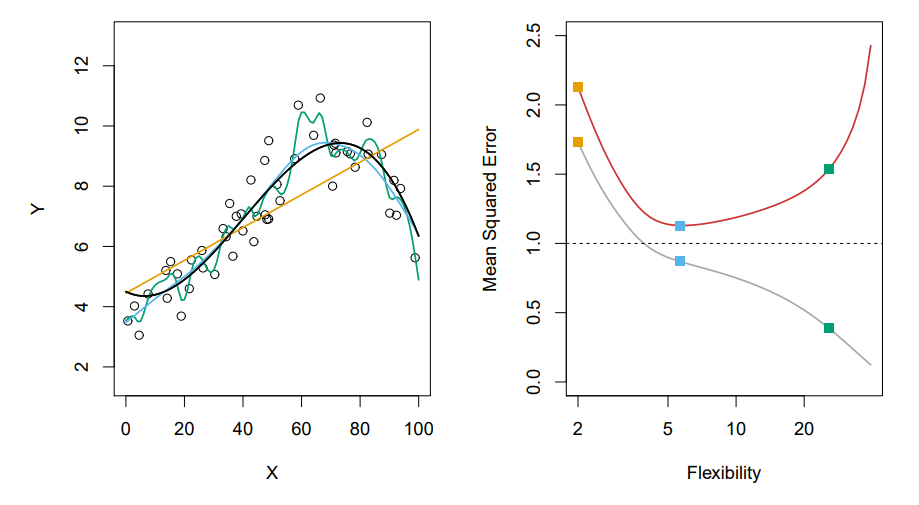
\includegraphics[width=8cm]{data/overfitting.png}
                    };
                }

                \only<4>{
                    \PythonInputNode{1}{(-4, 2)}{code}{0.9\textwidth}{7}{
                        import pandas as pd^^J
                        ^^J
                        ^^J
                        df = pd.read_csv('/Users/esten/Downloads/Auto.csv')^^J
                        train = df.iloc[:int(len(df) * 0.8)]^^J
                        validation = df.iloc[int(len(df) * 0.8):]^^J
                        ^^J
                        print(f'Using {len(train)} samples for training')^^J
                        print(f'Using {len(validation)} samples for validation')^^J
                    }
                    \PythonOutputNode{1}{($ (code.south west) + (0.11, -0.2) $)}{output}{0.791\textwidth}{7}{
                        Using 317 samples for training^^J
                        Using 80 samples for validation^^J
                    }
                }
            \end{tikzpicture}
        }
        \only<5>{
            \begin{enumerate}
                \item Variable selection
                \begin{enumerate}
                    \item[a.] Best subset selection
                    \item[b.] Forward stepwise selection
                    \item[c.] Backward stepwise selection
                \end{enumerate}
                \item Shrinkage
                \begin{enumerate}
                    \item[a.] LASSO
                    \item[b.] Ridge Regression
                \end{enumerate}
                \item Dimensionality reduction: Lecture 6 and self-study
            \end{enumerate}
        }
        \only<6>{
            \begin{enumerate}
                \item Variable selection
                \begin{enumerate}
                    \item[a.] Best subset selection
                    \item[b.] Forward stepwise selection
                    \item[c.] Backward stepwise selection
                \end{enumerate}
                \item Shrinkage
                \begin{enumerate}
                    \item[a.] \textcolor{red}{LASSO}
                    \item[b.] Ridge Regression
                \end{enumerate}
                \item Dimensionality reduction: Lecture 6 and self-study
            \end{enumerate}
        }
    \end{frame}

    \section{Variable selection}

    \newcommand{\autoplot}[1]{
        \nextgroupplot[
            title=\scriptsize{#1},
            every axis title/.style={at={(0.5,1.15)}}
        ]
            \addplot[
                only marks,
                mark=*,
                color=blue,
                opacity=0.25
            ] table[
                col sep=comma,
                y=mpg,
                x=#1
            ] {data/Auto.csv};
    }

    \newsavebox{\predictors}
    \sbox{\predictors}{
        \begin{tikzpicture}
            \begin{groupplot}[
                group style={
                    group size=3 by 2,
                    horizontal sep=0.5cm
                },
                ticklabel style = {font=\tiny},
                height=3.9cm,
                width=3.9cm
            ]
                \autoplot{cylinders}
                \autoplot{displacement}
                \autoplot{horsepower}
                \autoplot{weight}
                \autoplot{acceleration}
                \autoplot{year}
            \end{groupplot}
        \end{tikzpicture}
    }

    \begin{frame}{Variable selection}
        \begin{tikzpicture}
            \node[] at (-5.25, -3) {};
            \node[] at (5.25, 3) {};

            \only<1>{
                \node[align=center] at (0, 0) {
                    The number of predictors we are using in our model directly impacts model complexity.
                };
            }
            \only<2-3>{
                \node[align=left, anchor=west] at (-5.2, 2.5) {
                    \underline{Problem}\\
                    We have a set of predictors $P=\{x_0, x_1, ...\}$ and a target variable $y$, and we want to\\find the subset $p \subseteq P$ that yields the best (linear) model for predicting $y$.
                };
                \only<3>{
                    \node[align=left, anchor=west] at (-5.2, 1.2) {
                        \underline{Motivation}\\
                        To reduce model complexity (and therefore risk of overfitting), and to simplify\\subsequent interpretations.
                    };
                }
            }
            \only<4>{
                \node[] at (0, 0) {
                    \usebox{\predictors}
                };
            }
        \end{tikzpicture}
    \end{frame}


    \begin{frame}[t]{Variable selection: Best subset selection} % Implementation
        \only<1,3>{
            \underline{Problem}\\
            We have a set of predictors $P=\{x_0, x_1, ...\}$ and a target variable $y$, and we want to find the subset $p \subseteq P$ that yields the best (linear) model for predicting $y$.\\
            \vspace{0.25cm}
            \underline{Solution}\\
            Train models on all subsets $p$ and select the best one.\\
            \only<3>{
                \vspace{0.25cm}
                \underline{\textcolor{green}{+} Positives}\\
                Guaranteed to find the optimal solution.\\
                Simple implementation\\
                \vspace{0.25cm}
                \underline{\textcolor{red}{-} Drawbacks}\\
                Need to train many ($2^{|P|}$) models.
            }
        }
        \only<2>{
            \begin{tikzpicture}
                \node[] at (-5.25, -3) {};
                \node[] at (5.25, 3) {};

                \PythonInputNode{1}{(-5, 2.5)}{code}{0.95\textwidth}{6}{
import numpy as np^^J
^^J
from itertools import chain, combinations^^J
from sklearn.linear_model import LinearRegression^^J
^^J
subsets = list(chain.from_iterable(combinations(predictors, r) \^^J
{ }{ }{ }{ }{ }{ }{ }{ }{ }{ }{ }{ }{ }{ }{ }for r in range(len(predictors)+1)))^^J
^^J
best = {'mse': float('inf'), 'subset': None}^^J
^^J
for subset in subsets:^^J
{ }{ }{ }{ }if len(subset) == 0:^^J
{ }{ }{ }{ }{ }{ }{ }{ }continue^^J
^^J
{ }{ }{ }{ }model = LinearRegression()^^J
{ }{ }{ }{ }model.fit(train[list(subset)], train[target])^^J
{ }{ }{ }{ }predictions = model.predict(validation[list(subset)])^^J
{ }{ }{ }{ }mse = np.mean((predictions - validation[target]) ** 2)^^J
^^J
{ }{ }{ }{ }if mse < best['mse']:^^J
{ }{ }{ }{ }{ }{ }{ }{ }best = \{'mse': mse, 'subset': subset\}^^J
^^J
print(f'MSE: \{best["mse"]:.2f\}, predictors: \{best["subset"]\}')^^J
                }
                \PythonOutputNode{1}{($ (code.south west) + (0.11, -0.2) $)}{output}{0.881\textwidth}{6}{
MSE: 29.68, predictors: ('cylinders', 'displacement', 'horsepower', 'weight', 'year')^^J
                }
            \end{tikzpicture}
        }
        \only<4>{
            \centering
            \begin{tikzpicture}
                \begin{axis}[
                    smooth,
                    xmin=0,
                    xmax=10,
                    ymin=0,
                    ymax=1200,
                    xlabel={Number of predictors},
                    ylabel={Number of models},
                ]
                    \addplot[mark=*] coordinates {
                        (1, 2^1)
                        (2, 2^2)
                        (3, 2^3)
                        (4, 2^4)
                        (5, 2^5)
                        (6, 2^6)
                        (7, 2^7)
                        (8, 2^8)
                        (9, 2^9)
                        (10, 2^10)
                    };
                    \node[anchor=south] at (axis cs: 6, 2^6) {64};
                \end{axis}
            \end{tikzpicture}
        }
    \end{frame}

     \begin{frame}[t]{Variable selection: Forward stepwise selection}
        \only<1-9,12>{
            \underline{Problem}\\
            We have a set of predictors $P=\{x_0, x_1, ...\}$ and a target variable $y$, and we want to find the subset $p \subseteq P$ that yields the best (linear) model for predicting $y$.\\
            \vspace{0.25cm}
            \underline{Solution}\\
            Start with no predictors. Iteratively add the predictor that yields the best model until all are included.\\

            \only<12>{
                \vspace{0.25cm}
                \underline{\textcolor{green}{+} Positives}\\
                Need to train fewer models.\\
                \vspace{0.25cm}
                \underline{\textcolor{red}{-} Drawbacks}\\
                Not guaranteed to find the optimal solution.\\
            }
        }

        \only<2-9>{
            \def\nodefont{\fontsize{4}{4}\linespread{0.85}\selectfont}
            \def\hsep{1.6}
            \def\vsep{0.75}
            \begin{tikzpicture}
                \node[draw=black, align=center, font=\nodefont] (n00) at (0, 0 * \vsep) {
                    $y \sim \mathbbm{1}$\\
                    $mse=146.47$
                };

                \node[] at (6.5 * \hsep, 3.3 * \vsep) {};
                \node[] at (-0.32 * \hsep, -3.3 * \vsep) {};

                \only<3>{
                    \node[draw=black, align=center, font=\nodefont, color=black] (n11) at (\hsep, 2.5 * \vsep) {
                        $y \sim cylinders$\\
                        $67.96$
                    };
                    \node[draw=black, align=center, font=\nodefont, color=black] (n12) at (\hsep, 1.5 * \vsep) {
                        $y \sim year$\\
                        $61.56$
                    };
                    \node[draw=black, align=center, font=\nodefont, color=black] (n13) at (\hsep, 0.5 * \vsep) {
                        $y \sim acceleration$\\
                        $119.72$
                    };
                    \node[draw=black, align=center, font=\nodefont] (n14) at (\hsep, -0.5 * \vsep) {
                        $y \sim weight$\\
                        $61.18$
                    };
                    \node[draw=black, align=center, font=\nodefont, color=black] (n15) at (\hsep, -1.5 * \vsep) {
                        $y \sim horsepower$\\
                        $65.75$
                    };
                    \node[draw=black, align=center, font=\nodefont, color=black] (n16) at (\hsep, -2.5 * \vsep) {
                        $y \sim displacement$\\
                        $63.84$
                    };


                    \draw[black] (n00.east) -- (n11.west);
                    \draw[black] (n00.east) -- (n12.west);
                    \draw[black] (n00.east) -- (n13.west);
                    \draw[black] (n00.east) -- (n14.west);
                    \draw[black] (n00.east) -- (n15.west);
                    \draw[black] (n00.east) -- (n16.west);
                }
                \only<4-9>{
                    \node[draw=gray!25, align=center, font=\nodefont, color=gray!25] (n11) at (\hsep, 2.5 * \vsep) {
                        $y \sim cylinders$\\
                        $67.96$
                    };
                    \node[draw=gray!25, align=center, font=\nodefont, color=gray!25] (n12) at (\hsep, 1.5 * \vsep) {
                        $y \sim year$\\
                        $61.56$
                    };
                    \node[draw=gray!25, align=center, font=\nodefont, color=gray!25] (n13) at (\hsep, 0.5 * \vsep) {
                        $y \sim acceleration$\\
                        $119.72$
                    };
                    \node[draw=black, align=center, font=\nodefont] (n14) at (\hsep, -0.5 * \vsep) {
                        $y \sim weight$\\
                        $61.18$
                    };
                    \node[draw=gray!25, align=center, font=\nodefont, color=gray!25] (n15) at (\hsep, -1.5 * \vsep) {
                        $y \sim horsepower$\\
                        $65.75$
                    };
                    \node[draw=gray!25, align=center, font=\nodefont, color=gray!25] (n16) at (\hsep, -2.5 * \vsep) {
                        $y \sim displacement$\\
                        $63.84$
                    };


                    \draw[gray!25] (n00.east) -- (n11.west);
                    \draw[gray!25] (n00.east) -- (n12.west);
                    \draw[gray!25] (n00.east) -- (n13.west);
                    \draw[black] (n00.east) -- (n14.west);
                    \draw[gray!25] (n00.east) -- (n15.west);
                    \draw[gray!25] (n00.east) -- (n16.west);
                }
                \only<5>{
                    \node[draw=black, align=center, font=\nodefont, color=black] (n21) at (2 * \hsep, 2.5 * \vsep) {
                        $\begin{aligned}
                            y\sim&weight +\\[-0.8em]
                            &cylinders
                        \end{aligned}$\\
                        $60.02$
                    };
                    \node[draw=black, align=center, font=\nodefont] (n22) at (2 * \hsep, 1.25 * \vsep) {
                        $\begin{aligned}
                            y\sim&weight +\\[-0.8em]
                            &year
                        \end{aligned}$\\
                        $29.84$
                    };
                    \node[draw=black, align=center, font=\nodefont, color=black] (n23) at (2 * \hsep, 0 * \vsep) {
                        $\begin{aligned}
                            y\sim&weight +\\[-0.8em]
                            &acceleration
                        \end{aligned}$\\
                        $60.01$
                    };
                    \node[draw=black, align=center, font=\nodefont, color=black] (n24) at (2 * \hsep, -1.25 * \vsep) {
                        $\begin{aligned}
                            y\sim&weight +\\[-0.8em]
                            &horsepower
                        \end{aligned}$\\
                        $58.59$
                    };
                    \node[draw=black, align=center, font=\nodefont, color=black] (n25) at (2 * \hsep, -2.5 * \vsep) {
                        $\begin{aligned}
                            y\sim&weight +\\[-0.8em]
                            &displacement
                        \end{aligned}$\\
                        $59.91$
                    };

                    \draw[black] (n14.east) -- (n21.west);
                    \draw[black] (n14.east) -- (n22.west);
                    \draw[black] (n14.east) -- (n23.west);
                    \draw[black] (n14.east) -- (n24.west);
                    \draw[black] (n14.east) -- (n25.west);
                }
                \only<6-9>{
                    \node[draw=gray!25, align=center, font=\nodefont, color=gray!25] (n21) at (2 * \hsep, 2.5 * \vsep) {
                        $\begin{aligned}
                            y\sim&weight +\\[-0.8em]
                            &cylinders
                        \end{aligned}$\\
                        $60.02$
                    };
                    \node[draw=black, align=center, font=\nodefont] (n22) at (2 * \hsep, 1.25 * \vsep) {
                        $\begin{aligned}
                            y\sim&weight +\\[-0.8em]
                            &year
                        \end{aligned}$\\
                        $29.84$
                    };
                    \node[draw=gray!25, align=center, font=\nodefont, color=gray!25] (n23) at (2 * \hsep, 0 * \vsep) {
                        $\begin{aligned}
                            y\sim&weight +\\[-0.8em]
                            &acceleration
                        \end{aligned}$\\
                        $60.01$
                    };
                    \node[draw=gray!25, align=center, font=\nodefont, color=gray!25] (n24) at (2 * \hsep, -1.25 * \vsep) {
                        $\begin{aligned}
                            y\sim&weight +\\[-0.8em]
                            &horsepower
                        \end{aligned}$\\
                        $58.59$
                    };
                    \node[draw=gray!25, align=center, font=\nodefont, color=gray!25] (n25) at (2 * \hsep, -2.5 * \vsep) {
                        $\begin{aligned}
                            y\sim&weight +\\[-0.8em]
                            &displacement
                        \end{aligned}$\\
                        $59.91$
                    };

                    \draw[gray!25] (n14.east) -- (n21.west);
                    \draw[black] (n14.east) -- (n22.west);
                    \draw[gray!25] (n14.east) -- (n23.west);
                    \draw[gray!25] (n14.east) -- (n24.west);
                    \draw[gray!25] (n14.east) -- (n25.west);
                }
                \only<6>{
                    \node[draw=black, align=center, font=\nodefont, color=black] (n31) at (3 * \hsep, 2.25 * \vsep) {
                        $\begin{aligned}
                            y\sim&weight +\\[-0.8em]
                            &year +\\[-0.8em]
                            &cylinders
                        \end{aligned}$\\
                        $29.91$
                    };
                    \node[draw=black, align=center, font=\nodefont, color=black] (n32) at (3 * \hsep, 0.75 * \vsep) {
                        $\begin{aligned}
                            y\sim&weight +\\[-0.8em]
                            &year +\\[-0.8em]
                            &acceleration
                        \end{aligned}$\\
                        $29.99$
                    };
                    \node[draw=black, align=center, font=\nodefont] (n33) at (3 * \hsep, -0.75 * \vsep) {
                        $\begin{aligned}
                            y\sim&weight +\\[-0.8em]
                            &year +\\[-0.8em]
                            &horsepower
                        \end{aligned}$\\
                        $29.85$
                    };
                    \node[draw=black, align=center, font=\nodefont, color=black] (n34) at (3 * \hsep, -2.25 * \vsep) {
                        $\begin{aligned}
                            y\sim&weight +\\[-0.8em]
                            &year +\\[-0.8em]
                            &displacement
                        \end{aligned}$\\
                        $29.96$
                    };

                    \draw[black] (n22.east) -- (n31.west);
                    \draw[black] (n22.east) -- (n32.west);
                    \draw[black] (n22.east) -- (n33.west);
                    \draw[black] (n22.east) -- (n34.west);
                }
                \only<7-9>{
                    \node[draw=gray!25, align=center, font=\nodefont, color=gray!25] (n31) at (3 * \hsep, 2.25 * \vsep) {
                        $\begin{aligned}
                            y\sim&weight +\\[-0.8em]
                            &year +\\[-0.8em]
                            &cylinders
                        \end{aligned}$\\
                        $29.91$
                    };
                    \node[draw=gray!25, align=center, font=\nodefont, color=gray!25] (n32) at (3 * \hsep, 0.75 * \vsep) {
                        $\begin{aligned}
                            y\sim&weight +\\[-0.8em]
                            &year +\\[-0.8em]
                            &acceleration
                        \end{aligned}$\\
                        $29.99$
                    };
                    \node[draw=black, align=center, font=\nodefont] (n33) at (3 * \hsep, -0.75 * \vsep) {
                        $\begin{aligned}
                            y\sim&weight +\\[-0.8em]
                            &year +\\[-0.8em]
                            &horsepower
                        \end{aligned}$\\
                        $29.85$
                    };
                    \node[draw=gray!25, align=center, font=\nodefont, color=gray!25] (n34) at (3 * \hsep, -2.25 * \vsep) {
                        $\begin{aligned}
                            y\sim&weight +\\[-0.8em]
                            &year +\\[-0.8em]
                            &displacement
                        \end{aligned}$\\
                        $29.96$
                    };

                    \draw[gray!25] (n22.east) -- (n31.west);
                    \draw[gray!25] (n22.east) -- (n32.west);
                    \draw[black] (n22.east) -- (n33.west);
                    \draw[gray!25] (n22.east) -- (n34.west);
                }
                \only<7>{
                    \node[draw=black, align=center, font=\nodefont, color=black] (n41) at (4 * \hsep, 1.75 * \vsep) {
                        $\begin{aligned}
                            y\sim&weight +\\[-0.8em]
                            &year +\\[-0.8em]
                            &horsepower +\\[-0.8em]
                            &cylinders
                        \end{aligned}$\\
                        $29.87$
                    };
                    \node[draw=black, align=center, font=\nodefont, color=black] (n42) at (4 * \hsep, 0 * \vsep) {
                        $\begin{aligned}
                            y\sim&weight +\\[-0.8em]
                            &year +\\[-0.8em]
                            &horsepower +\\[-0.8em]
                            &acceleration
                        \end{aligned}$\\
                        $30.29$
                    };
                    \node[draw=black, align=center, font=\nodefont, color=black] (n43) at (4 * \hsep, -1.75 * \vsep) {
                        $\begin{aligned}
                            y\sim&weight +\\[-0.8em]
                            &year +\\[-0.8em]
                            &horsepower +\\[-0.8em]
                            &displacement
                        \end{aligned}$\\
                        $29.95$
                    };

                    \draw[black] (n33.east) -- (n41.west);
                    \draw[black] (n33.east) -- (n42.west);
                    \draw[black] (n33.east) -- (n43.west);
                }
                \only<8-9>{
                    \node[draw=black, align=center, font=\nodefont, color=black] (n41) at (4 * \hsep, 1.75 * \vsep) {
                        $\begin{aligned}
                            y\sim&weight +\\[-0.8em]
                            &year +\\[-0.8em]
                            &horsepower +\\[-0.8em]
                            &cylinders
                        \end{aligned}$\\
                        $29.87$
                    };
                    \node[draw=gray!25, align=center, font=\nodefont, color=gray!25] (n42) at (4 * \hsep, 0 * \vsep) {
                        $\begin{aligned}
                            y\sim&weight +\\[-0.8em]
                            &year +\\[-0.8em]
                            &horsepower +\\[-0.8em]
                            &acceleration
                        \end{aligned}$\\
                        $30.29$
                    };
                    \node[draw=gray!25, align=center, font=\nodefont, color=gray!25] (n43) at (4 * \hsep, -1.75 * \vsep) {
                        $\begin{aligned}
                            y\sim&weight +\\[-0.8em]
                            &year +\\[-0.8em]
                            &horsepower +\\[-0.8em]
                            &displacement
                        \end{aligned}$\\
                        $29.95$
                    };

                    \draw[black] (n33.east) -- (n41.west);
                    \draw[gray!25] (n33.east) -- (n42.west);
                    \draw[gray!25] (n33.east) -- (n43.west);
                }
                \only<8>{
                    \node[draw=black, align=center, font=\nodefont] (n51) at (5 * \hsep, 1 * \vsep) {
                        $\begin{aligned}
                            y\sim&weight +\\[-0.8em]
                            &year +\\[-0.8em]
                            &horsepower +\\[-0.8em]
                            &cylinders +\\[-0.8em]
                            &acceleration
                        \end{aligned}$\\
                        $29.68$
                    };
                    \node[draw=black, align=center, font=\nodefont, color=black] (n52) at (5 * \hsep, -1 * \vsep) {
                        $\begin{aligned}
                            y\sim&weight +\\[-0.8em]
                            &year +\\[-0.8em]
                            &horsepower +\\[-0.8em]
                            &cylinders +\\[-0.8em]
                            &displacement
                        \end{aligned}$\\
                        $30.47$
                    };

                    \draw[black] (n41.east) -- (n51.west);
                    \draw[black] (n41.east) -- (n52.west);
                }
                \only<9>{
                    \node[draw=black, align=center, font=\nodefont] (n51) at (5 * \hsep, 1 * \vsep) {
                        $\begin{aligned}
                            y\sim&weight +\\[-0.8em]
                            &year +\\[-0.8em]
                            &horsepower +\\[-0.8em]
                            &cylinders +\\[-0.8em]
                            &acceleration
                        \end{aligned}$\\
                        $29.68$
                    };
                    \node[draw=gray!25, align=center, font=\nodefont, color=gray!25] (n52) at (5 * \hsep, -1 * \vsep) {
                        $\begin{aligned}
                            y\sim&weight +\\[-0.8em]
                            &year +\\[-0.8em]
                            &horsepower +\\[-0.8em]
                            &cylinders +\\[-0.8em]
                            &displacement
                        \end{aligned}$\\
                        $30.47$
                    };

                    \draw[black] (n41.east) -- (n51.west);
                    \draw[gray!25] (n41.east) -- (n52.west);

                    \node[draw=black, align=center, font=\nodefont] (n61) at (6 * \hsep, 0 * \vsep) {
                        $\begin{aligned}
                            y\sim&weight +\\[-0.8em]
                            &year +\\[-0.8em]
                            &horsepower +\\[-0.8em]
                            &cylinders +\\[-0.8em]
                            &acceleration +\\[-0.8em]
                            &displacement
                        \end{aligned}$\\
                        $30.29$
                    };

                    \draw[black] (n51.east) -- (n61.west);
                }
            \end{tikzpicture}
        }
        \only<10>{
            \centering
            \vspace{0.7cm}
            \begin{tikzpicture}
                \begin{axis}[
                    xmin=-0.5,
                    xmax=6.5,
                    ymin=0,
                    ymax=150,
                    ytick pos=left,
                    xtick pos=bottom,
                    ylabel=MSE,
                    xlabel=Number of predictors
                ]
                    \addplot[red,mark=*] coordinates {
                        (0, 44.74)
                        (1, 11.02)
                        (2, 8.31)
                        (3, 8.31)
                        (4, 8.25)
                        (5, 8.24)
                        (6, 8.21)
                    };
                    \addplot[blue,mark=*] coordinates {
                        (0, 146.47)
                        (1, 61.18)
                        (2, 29.84)
                        (3, 29.85)
                        (4, 29.87)
                        (5, 29.68)
                        (6, 30.29)
                    };

                    \node[
                        circle,
                        fill=red,
                        minimum size=4.3pt,
                        inner sep=0pt,
                        label=right:Training
                    ] at (axis cs: 4.7, 140) {};
                    \node[
                        circle,
                        fill=blue,
                        minimum size=4.3pt,
                        inner sep=0pt,
                        label=right:Validation
                    ] at (axis cs: 4.7, 132) {};

                    \node[anchor=west,font=\small] at (axis cs: 0, 44.74) {44.74};
                    \node[anchor=south west,font=\small] at (axis cs: 1, 11.02) {11.02};
                    \node[anchor=south,font=\small] at (axis cs: 2, 8.31) {8.31};
                    \node[anchor=south,font=\small] at (axis cs: 3, 8.31) {8.30};
                    \node[anchor=south,font=\small] at (axis cs: 4, 8.25) {8.25};
                    \node[anchor=south,font=\small] at (axis cs: 5, 8.24) {8.24};
                    \node[anchor=south,font=\small] at (axis cs: 6, 8.21) {8.21};

                    \node[anchor=west,font=\small] at (axis cs: 0, 146.47) {146.47};
                    \node[anchor=west,font=\small] at (axis cs: 1, 61.18) {61.18};
                    \node[anchor=south west,font=\small] at (axis cs: 2, 29.84) {29.84};
                    \node[anchor=south,font=\small] at (axis cs: 3, 29.85) {29.85};
                    \node[anchor=south,font=\small] at (axis cs: 4, 29.87) {29.87};
                    \node[anchor=south,font=\small] at (axis cs: 5, 29.68) {29.68};
                    \node[anchor=south,font=\small] at (axis cs: 6, 30.29) {30.29};

                \end{axis}
            \end{tikzpicture}
        }
        \only<11>{
            \begin{tikzpicture}
                \node[] at (-5.25, -3) {};
                \node[] at (5.25, 3) {};

                \PythonInputNode{1}{(-5, 2.5)}{code}{0.95\textwidth}{4}{
def fit_and_evaluate(train: pd.DataFrame, validation: pd.DataFrame,^^J
{ }{ }{ }{ }{ }{ }{ }{ }{ }{ }{ }{ }{ }{ }{ }{ }{ }{ }{ }{ }{ }predictors: List[str], target: str):^^J
{ }{ }{ }{ }model = LinearRegression()^^J
{ }{ }{ }{ }model.fit(train[predictors], train[target])^^J
   ^^J
{ }{ }{ }{ }train_predictions = model.predict(train[predictors])^^J
{ }{ }{ }{ }validation_predictions = model.predict(validation[predictors])^^J
^^J
{ }{ }{ }{ }return np.mean((train_predictions - train[target]) ** 2), \^^J
{ }{ }{ }{ }{ }{ }{ }{ }{ }{ }{ }np.mean((validation_predictions - validation[target]) ** 2)^^J
^^J
^^J
predictors = ['cylinders', 'displacement', 'horsepower', 'weight', 'acceleration', 'year']^^J
target = 'mpg'^^J
^^J
train['intercept'] = 1^^J
validation['intercept'] = 1^^J
train_mse, validation_mse = fit_and_evaluate(train, validation, predictors=['intercept'], target=target)^^J
print(f'[]: \{validation_mse:.2f\} (\{train_mse:.2f\})')^^J
^^J
chosen_predictors = []^^J
^^J
while len(chosen_predictors) < len(predictors):^^J
{ }{ }{ }{ }best_predictor = \{'train_mse': None, 'validation_mse': float('inf'),^^J
{ }{ }{ }{ }{ }{ }{ }{ }{ }{ }{ }{ }{ }{ }{ }{ }{ }{ }{ }{ }{ }{ }'predictor': None\}^^J
          ^^J
{ }{ }{ }{ }for predictor in set(predictors) - set(chosen_predictors):^^J
{ }{ }{ }{ }{ }{ }{ }{ }train_mse, validation_mse = fit_and_evaluate(train, validation, predictors=chosen_predictors + [predictor], target=target)^^J
^^J
{ }{ }{ }{ }{ }{ }{ }{ }if validation_mse < best_predictor['validation_mse']:^^J
{ }{ }{ }{ }{ }{ }{ }{ }{ }{ }{ }{ }best_predictor = \{'train_mse': train_mse, 'validation_mse': validation_mse, 'predictor': predictor\}^^J
^^J
{ }{ }{ }{ }chosen_predictors.append(best_predictor['predictor'])^^J
^^J
{ }{ }{ }{ }print(f'\{chosen_predictors\}: \{best_predictor["validation_mse"]:.2f\} (\{best_predictor["train_mse"]:.2f\})')^^J
                }
            \end{tikzpicture}
        }
    \end{frame}

    \begin{frame}[t]{Variable selection: Backward stepwise selection}
        \underline{Problem}\\
        We have a set of predictors $P=\{x_0, x_1, ...\}$ and a target variable $y$, and we want to find the subset $p \subseteq P$ that yields the best (linear) model for predicting $y$.\\
        \vspace{0.25cm}
        \underline{Solution}\\
        Start with all predictors. Iteratively remove the predictor that yields the best model until all you have none left.\\
        \only<2>{
            \vspace{0.25cm}
            \underline{\textcolor{green}{+} Positives}\\
            Need to train fewer models.\\
            \vspace{0.25cm}
            \underline{\textcolor{red}{-} Drawbacks}\\
            Not guaranteed to find the optimal solution.\\
        }
    \end{frame}

    \section{Shrinkage}

    \def\codewidth{5.2cm}

    \begin{frame}{Shrinkage: Outline}
        \definecolor{mse}{HTML}{cc79a7}
        \definecolor{variance}{HTML}{10a47b}
        \begin{tikzpicture}
            \node[] at (-5.25, 3.5) {};
            \node[] at (5.25, -3.5) {};

            \only<1>{
                \node[] at (0, 3) {
                    $y \sim \beta_0 + $
                    $\beta_1$$x_1 + $
                    $\beta_2$$x_2 + $
                    $\beta_3$$x_3 + $
                    $\beta_4$$x_4 + $
                    $\beta_5$$x_5 + $
                    $\beta_6$$x_6$
                };
            }
            \only<2-9>{
                \node[] at (0, 3) {
                    $y \sim \beta_0 + $
                    \textcolor{red}{$\beta_1$}$x_1 + $
                    \textcolor{red}{$\beta_2$}$x_2 + $
                    \textcolor{red}{$\beta_3$}$x_3 + $
                    \textcolor{red}{$\beta_4$}$x_4 + $
                    \textcolor{red}{$\beta_5$}$x_5 + $
                    \textcolor{red}{$\beta_6$}$x_6$
                };
            }
            \only<3-9>{
                \node[] at (0, 2.5) {
                    \textcolor{red}{$\beta_n \rightarrow 0$}
                };
            }
            \only<4-6>{
                \node[anchor=north west, align=left, text width=8cm] at (-4.1, 2) {
                    \begin{enumerate}
                        \item $\beta_1 = 0 \implies \text{One less degree of freedom in our function}$\\
                    \end{enumerate}
                };
            }
            \only<5>{
                \node[] at (0, -3) {
                    $mse$$ = $$bias^2$$ + $$variance$$ + irreducible\ error$
                };
            }
            \only<6>{
                \node[] at (0, -3) {
                    \textcolor{mse}{$mse$}$ = $$bias^2$$ + $\textcolor{variance}{$variance$}\textcolor{gray!25}{$ + irreducible\ error$}
                };
                \node[inner sep=0pt, draw=black] at (0, -0.7) {
                    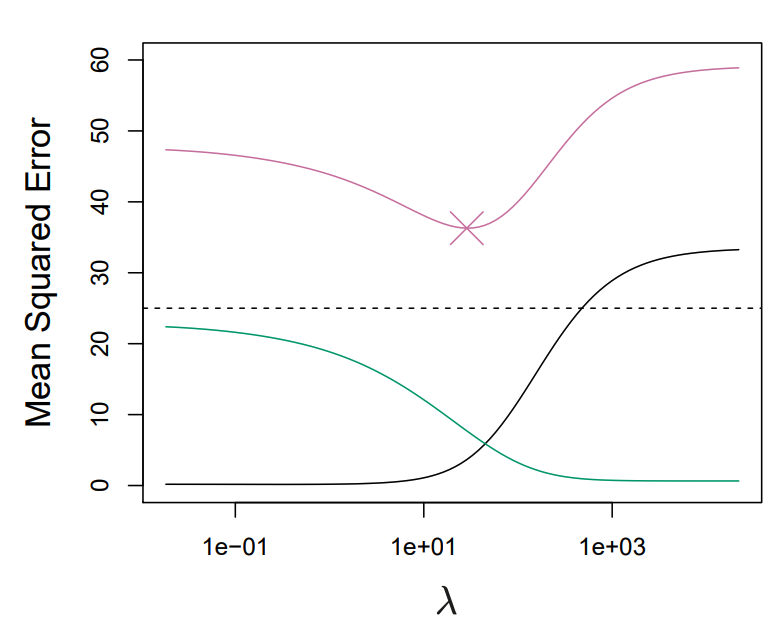
\includegraphics[width=4.5cm]{data/bias_variance_decomp.png}
                };
            }

            \only<7-8>{
                \node[anchor=north west, align=left, text width=8cm] at (-4.1, 2) {
                    \begin{enumerate}
                        \item $\beta_1 = 0 \implies \text{One less degree of freedom in our function}$\\
                        \item $\text{A little more bias} \implies \text{A lot less variance}$\\
                    \end{enumerate}
                };
            }

            \only<8>{
                \node[] (formula) at (0, -0.7) {
                    $y \sim \beta_0 + $
                    $\beta_1$$x_1 + $
                    $\beta_2$$x_2 + $
                    $\beta_3$$x_3 + $
                    $\beta_4$$x_4 + $
                    $\beta_5$$x_5 + $
                    $\beta_6$$x_6$
                };
                \draw[-stealth] ($ (formula.north) + (-0.9, 0) $) -- ($ (formula.north) + (-0.9, 0.3) $);
                \draw[-stealth] ($ (formula.south) - (-0.86, 0) $) -- ($ (formula.south) - (-0.86, 0.3) $);
            }

            \only<9>{
                \node[anchor=north west, align=left, text width=8cm] at (-4.1, 2) {
                    \begin{enumerate}
                        \item $\beta_1 = 0 \implies \text{One less degree of freedom in our function}$\\
                        \item $\text{A little more bias} \implies \text{A lot less variance}$\\
                        \item $\text{Parameters depend on eachother} \implies \text{Fewer degrees of freedom}$
                    \end{enumerate}
                };
            }
        \end{tikzpicture}
    \end{frame}

    \begin{frame}{Shrinkage: Ridge regression} % MSE
        \begin{tikzpicture}
            \node[] at (-5.25, -3) {};
            \node[] at (5.25, 3) {};

            \only<1>{
                \node[inner sep=0pt, anchor=west] (loss) at (-2, 0) {
                    $= \sum\limits_{i=0}^n \left( y_i - \sum\limits_{j=0}^p \beta_j x_{ij} \right)^2$
                };
                \node[anchor=east, inner sep=0pt] at (loss.west) {
                    $loss_{mse}$
                };
            }
            \only<2,5>{
                \node[inner sep=0pt, anchor=west] (loss) at (-2, 0) {
                    $= \sum\limits_{i=0}^n \left( y_i - \sum\limits_{j=0}^p \beta_j x_{ij} \right)^2$
                };
                \node[anchor=west, inner sep=0pt] (ridge) at (loss.east) {
                    $ + \lambda \sum\limits_{j=0}^p \beta_j^2$
                };
                \node[anchor=east, inner sep=0pt] at (loss.west) {
                    $loss_{ridge}$
                };
            }
            \only<3>{
                \node[inner sep=0pt, anchor=west] (loss) at (-2, 0) {
                    $= \sum\limits_{i=0}^n \left( y_i - \sum\limits_{j=0}^p \beta_j x_{ij} \right)^2$
                };
                \node[anchor=west, inner sep=0pt, draw=red] (ridge) at (loss.east) {
                    $ + \lambda \sum\limits_{j=0}^p \beta_j^2$
                };
                \node[anchor=east, inner sep=0pt] at (loss.west) {
                    $loss_{ridge}$
                };

                \draw[double, -Latex, red] ($ (ridge.south) - (0, 0.2) $) -- ($ (ridge.south) - (0, 0.6) $);
                \node[red] at ($ (ridge.south) - (0, 0.8) $) {
                    $\lambda \to \infty \Rightarrow \beta \to 0$
                };
            }
            \only<4>{
                \node[draw=black, fill=white] {
                    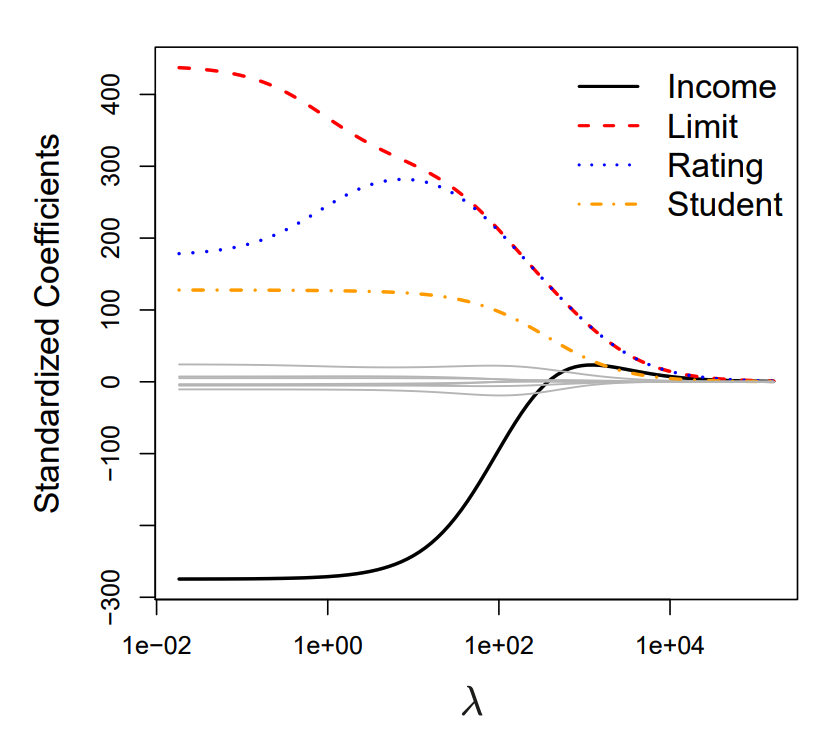
\includegraphics[width=8cm]{data/ridge_coefs.png}
                };
            }
            \only<5>{
                \node[] at (0, -1.5) {
                    $y \sim \beta0 + \beta_1x_1 + \beta_2x_2, x_1 \in [0, 1], x_2 \in [0, 1000]$
                };
            }

        \end{tikzpicture}
    \end{frame}

    \newsavebox{\predictorscales}
    \sbox{\predictorscales}{
        \begin{tikzpicture}
            \begin{axis}[
                width=6cm,
                height=6cm,
                xlabel=Acceleration,
                ylabel=Weight
            ]
                \addplot[only marks, blue!50, opacity=0.5] table [col sep=comma, x=acceleration, y=weight] {data/Auto.csv};
            \end{axis}
        \end{tikzpicture}
    }

    \begin{frame}{Shrinkage: Feature standardization}
        \begin{tikzpicture}
            \node[] at (-5.4, -4) {};
            \node[] at (5.4, 3) {};

            \only<1>{
                \node[] at (0, 0) {
                    \usebox{\predictorscales}
                };
            }
            \only<2-4>{
                \node[] at (0, 3) {\underline{\textbf{z-score standardization}}};

                \only<3-4>{
                    \node[] at (0, 2.3) {
                        $\mathbf{x} = \frac{\mathbf{x} - \mu_x}{\sigma_x}$
                    };
                }
                \only<4-4>{
                    \PythonInputNode{1}{(-4.5, 1.5)}{pythonnode}{0.95\textwidth}{7}{
for col in predictors:^^J
{ }{ }{ }{ }print(f'\{col\}: \{np.mean(df[col]):.2f\} (\{np.std(df[col]):.2f\})')^^J
^^J
\# z-score standardization^^J
for col in predictors:^^J
{ }{ }{ }{ }df[col] = (df[col] - np.mean(df[col])) / np.std(df[col])^^J
^^J
for col in predictors:^^J
{ }{ }{ }{ }print(f'\{col\} after: \{np.mean(df[col]):.2f\} (\{np.std(df[col]):.2f\})')^^J
                    }
                    \PythonOutputNode{1}{(-4.39, -1.2)}{output}{0.882\textwidth}{7}{
cylinders: 5.47 (1.70)^^J
displacement: 194.41 (104.51)^^J
horsepower: 104.47 (38.44)^^J
cylinders after: -0.00 (1.00)^^J
displacement after: -0.00 (1.00)^^J
horsepower after: -0.00 (1.00)^^J
                    }
                }
            }
        \end{tikzpicture}
    \end{frame}

    \begin{frame}{Shrinkage: Ridge regression}
        \begin{tikzpicture}
            \node[] at (-5.25, -3) {};
            \node[] at (5.25, 3) {};

            \node[inner sep=0pt] (loss) at (0, 0) {
                $= \sum\limits_{i=0}^n \left( y_i - \sum\limits_{j=0}^p \beta_j x_{ij} \right)^2$
            };
            \node[anchor=west, inner sep=0pt] (ridge) at (loss.east) {
                $ + \lambda \sum\limits_{j=0}^p$$\beta_j^2$
            };
            \node[anchor=east, inner sep=0pt] at (loss.west) {
                $loss_{ridge}$
            };

            \only<2>{
                \node[rotate=45] at (0, 0) {
                    \textcolor{red}{\Huge{Blackboard!}}
                };
            }

            \only<3>{
                \node[] at (0, -1.5) {
                    \url{http://localhost:8888/notebooks/notebooks/Live\%20coding.ipynb}
                };
            }

            \only<4>{
                \node[] at (0, -1.5) {
                    Regularization by shrinking the model covariates towards zero.
                };
            }
        \end{tikzpicture}
    \end{frame}

    \begin{frame}{Shrinkage: LASSO}
        \begin{tikzpicture}
            \node[] at (-5.25, -3.5) {};
            \node[] at (5.25, 3.5) {};

            \only<1-2>{
                \node[inner sep=0pt] (loss) at (0, 0) {
                    $= \sum\limits_{i=0}^n \left( y_i - \sum\limits_{j=0}^p \beta_j x_{ij} \right)^2$
                };
                \only<1>{
                    \node[anchor=west, inner sep=0pt] (ridge) at (loss.east) {
                        $ + \lambda \sum\limits_{j=0}^p$$\beta_j^2$
                    };
                }
                \only<2>{
                    \node[anchor=west, inner sep=0pt] (ridge) at (loss.east) {
                        $ + \lambda \sum\limits_{j=0}^p$\textcolor{red}{$\beta_j^2$}
                    };
                }
                \node[anchor=east, inner sep=0pt] at (loss.west) {
                    $loss_{ridge}$
                };

                \node[inner sep=0pt] (lassomse) at (0, -1.5) {
                    $= \sum\limits_{i=0}^n \left( y_i - \sum\limits_{j=0}^p \beta_j x_{ij} \right)^2$
                };
                \only<1>{
                    \node[anchor=west, inner sep=0pt] (lasso) at (lassomse.east) {
                        $ + \lambda \sum\limits_{j=0}^p$$|\beta_j|$
                    };
                }
                \only<2>{
                    \node[anchor=west, inner sep=0pt] (lasso) at (lassomse.east) {
                        $ + \lambda \sum\limits_{j=0}^p$\textcolor{red}{$|\beta_j|$}
                    };
                }
                \node[anchor=east, inner sep=0pt] at (lassomse.west) {
                    $loss_{lasso}$
                };
            }
            \only<3-5>{
                \node[fill=white, draw=black, label=Ridge] at (-2.5, 1) {
                    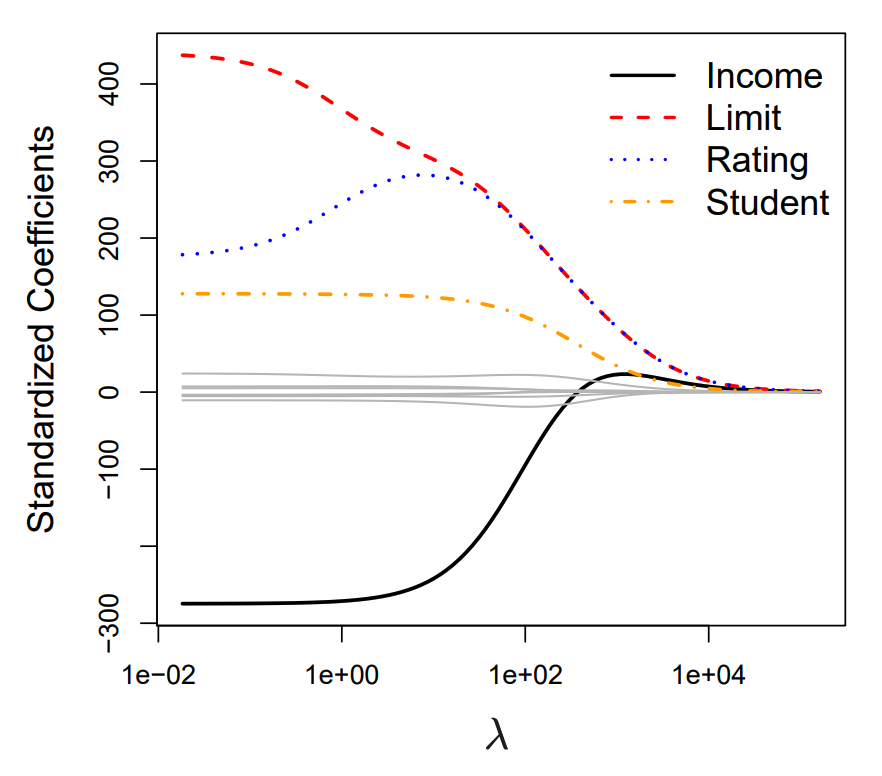
\includegraphics[width=3cm]{data/ridge.png}
                };
                \node[fill=white, draw=black, label=LASSO] at (2.5, 1) {
                    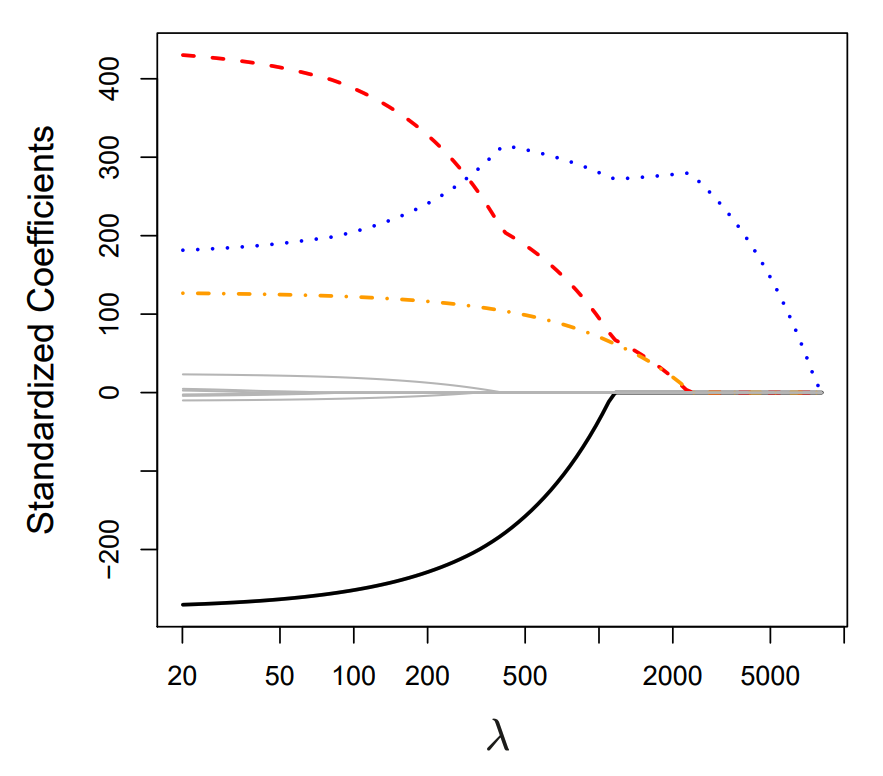
\includegraphics[width=3cm]{data/lasso.png}
                };

                \only<4>{
                    \node[] at (0, -2) {
                        \begin{tabular}{|c|c|c|}
                            \hline
                            \textbf{Predictor}&\textbf{Ridge}&\textbf{LASSO}\\
                            \hline
                            Intercept&23.44&23.44\\
                            \hline
                            Weight&-5.59&-4.78\\
                            \hline
                            Year&2.75&2.00\\
                            \hline
                            Acceleration&0.19&0\\
                            \hline
                            Displacement&0.66&0\\
                            \hline
                        \end{tabular}
                    };
                }
                \only<5>{
                    \node[align=center,red,font=\bfseries] at (0, -2) {
                        A coefficient of 0 does not mean the predictor has\\no association with the outcome!
                    };
                }
            }
            \only<6>{
                \node[fill=white, draw=black, anchor=east] (intuition) at (4.3, 0) {
                    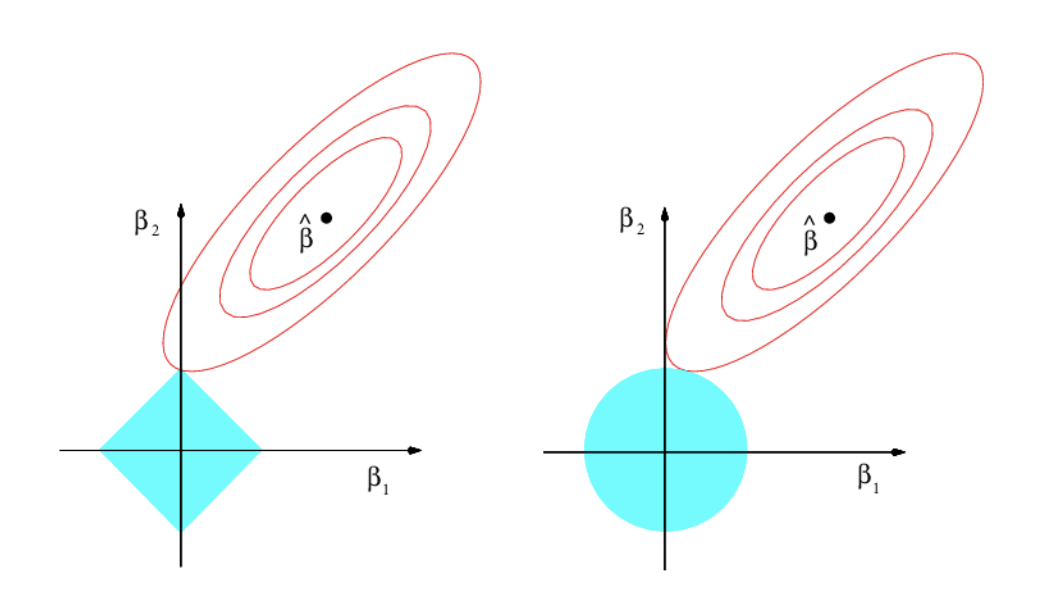
\includegraphics[
                        height=5cm,
                        trim={9cm 0 0 0},
                        clip
                    ]{data/lasso_intuition.png}
                };
                \node[anchor=south, text depth=0] at ($ (intuition.north east) - (2.3, 0) $) {Ridge};
                \node[anchor=south, text depth=0] at ($ (intuition.north east) - (6.3, 0) $) {Lasso};
                \node[font=\Huge\selectfont] at ($ (intuition.east) - (6.3, 0) $) {?};
                \node[] at (0, -3) {
                    \Large{Whiteboard!} \emoji{partying-face}
                };
            }
            \only<7>{
                \node[fill=white, draw=black, anchor=east] (intuition) at (4.3, 0) {
                    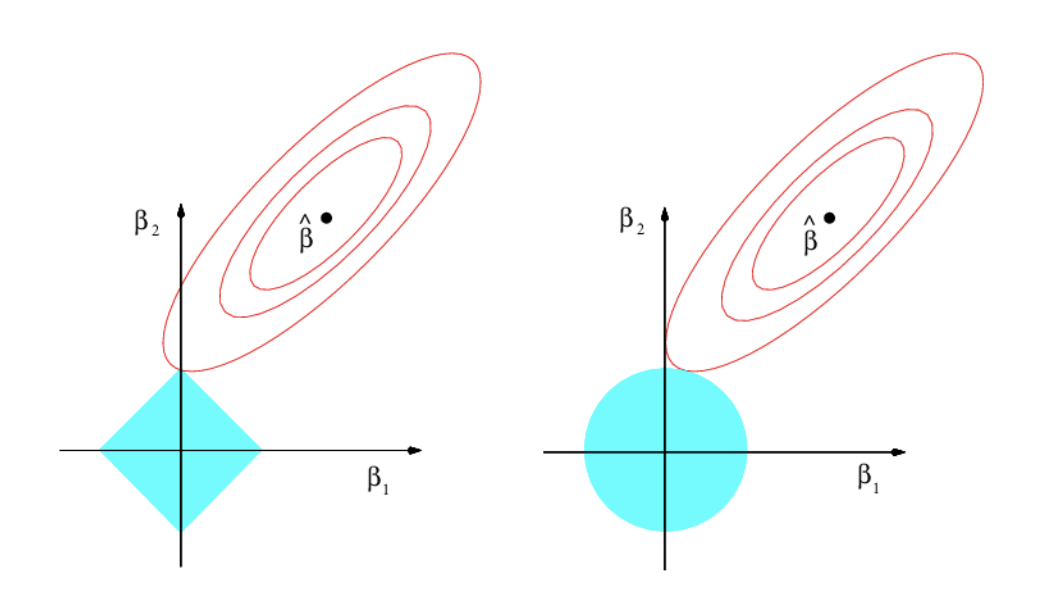
\includegraphics[
                        height=5cm
                    ]{data/lasso_intuition.png}
                };
                \node[anchor=south, text depth=0] at ($ (intuition.north east) - (2.3, 0) $) {Ridge};
                \node[anchor=south, text depth=0] at ($ (intuition.north east) - (6.3, 0) $) {Lasso};
            }
            \only<8>{
                \node[fill=white, draw=black] at (0, 0) {
                    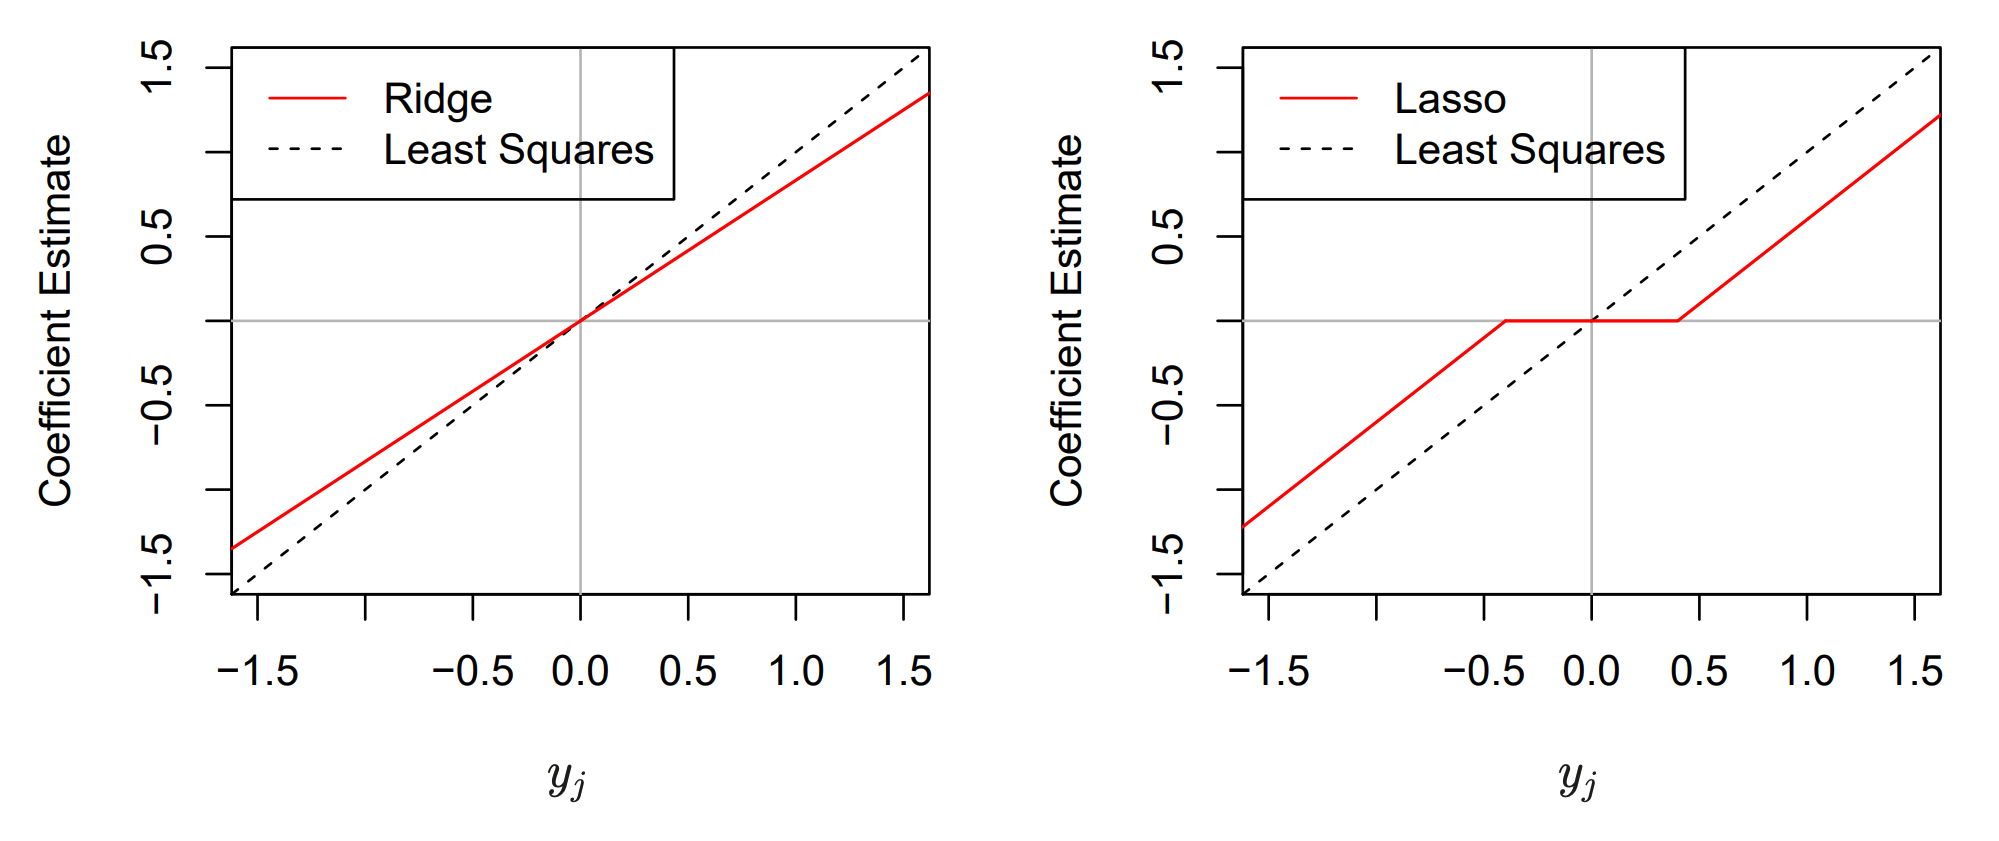
\includegraphics[width=10cm]{data/ridge_vs_lasso.png}
                };
            }
        \end{tikzpicture}
    \end{frame}


    \begin{frame}{Shrinkage: Summary} % LASSO
        \centering
        \vfill
        \begin{tikzpicture}
            \node[] at (-3, -4) {};
            \node[] at (6.8, 3) {};

            \draw[black] (3.2, 3) -- (3.2, -3.9);

            \node[inner sep=0pt] (mse) at (0, 2.2) {
                $= \sum\limits_{i=0}^n \left( y_i - \sum\limits_{j=0}^p \beta_j x_{ij} \right)^2$
            };
            \node[anchor=east, inner sep=0pt] at (mse.west) {
                $loss_{mse}$
            };
            \node[anchor=west, align=left] at ($ (mse.west) + (4.7, 0) $) {Fits the \textbf{best} model\\to the data.};

            \only<2-3>{
                \node[inner sep=0pt] (ridgemse) at (0, 0) {
                    $= \sum\limits_{i=0}^n \left( y_i - \sum\limits_{j=0}^p \beta_j x_{ij} \right)^2$
                };
                \node[anchor=west, inner sep=0pt] (lasso) at (ridgemse.east) {
                    $ + \lambda \sum\limits_{j=0}^p \beta_j^2$
                };
                \node[anchor=east, inner sep=0pt] at (ridgemse.west) {
                    $loss_{ridge}$
                };
                \node[anchor=west, align=left] at ($ (ridgemse.west) + (4.7, 0) $) {Fits the \textbf{best} model\\to the data while\\\textbf{shrinking} coefficients\\towards zero.};
            }

            \only<3>{
                \node[inner sep=0pt] (lassomse) at (0, -2.2) {
                    $= \sum\limits_{i=0}^n \left( y_i - \sum\limits_{j=0}^p \beta_j x_{ij} \right)^2$
                };
                \node[anchor=west, inner sep=0pt] (lasso) at (lassomse.east) {
                    $ + \lambda \sum\limits_{j=0}^p |\beta_j|$
                };
                \node[anchor=east, inner sep=0pt] at (lassomse.west) {
                    $loss_{lasso}$
                };

                \node[anchor=west, align=left] at ($ (lassomse.west) + (4.7, 0) $) {Fits the \textbf{best} model\\to the data while\\\textbf{shrinking} coefficients\\towards zero such\\that some variables\\are effectively \textbf{removed}.};
            }
        \end{tikzpicture}
        \vfill
    \end{frame}

    \section{Assignment 3}

    \begin{frame}{Assignment 3}
        \footnotesize{\url{https://uio.instructure.com/courses/53357/assignments/118667?module_item_id=962921}}
    \end{frame}

    \begin{frame}{Coding tips: Separation of concerns} % Spaghetti
        \centering
        \begin{tikzpicture}
            \node[] at (0, -7.55) {};
            \only<1-2>{
                \PythonInputNode{1}{(0, 0)}{code}{0.9\textwidth}{4}{
\# Read and clean data^^J
path = '/Users/esten/Downloads/Auto.csv'^^J
df = pd.read_csv(path)^^J
^^J
\# Split data^^J
train = df.iloc[:int(len(df) * 0.8)]^^J
validation = df.iloc[int(len(df) * 0.8):]^^J
^^J
\# Define input and output variables^^J
predictors = ['cylinders', 'displacement', 'horsepower', 'weight', 'acceleration', 'year']^^J
target = 'mpg'^^J
^^J
\# Define necessary data structures for state^^J
chosen_predictors = []^^J
mses = []^^J
^^J
while len(predictors) > 0:^^J
{ }{ }{ }{ }best_predictor = \{'mse': float('inf'), 'predictor': None\}^^J
^^J
{ }{ }{ }{ }for predictor in set(predictors) - set(chosen_predictors):^^J
{ }{ }{ }{ }{ }{ }{ }{ }potential_predictors = chosen_predictors + [predictor]^^J
^^J
{ }{ }{ }{ }{ }{ }{ }{ }\# Fit and evaluate model^^J
{ }{ }{ }{ }{ }{ }{ }{ }model = LinearRegression()^^J
{ }{ }{ }{ }{ }{ }{ }{ }model.fit(train[potential_predictors], train[target])^^J
{ }{ }{ }{ }{ }{ }{ }{ }predictions = model.predict(validation[potential_predictors])^^J
{ }{ }{ }{ }{ }{ }{ }{ }test_mse = np.mean((validation[target] - predictions) ** 2)^^J
^^J
{ }{ }{ }{ }{ }{ }{ }{ }\# Compare model with previous best^^J
{ }{ }{ }{ }{ }{ }{ }{ }if test_mse < best_predictor['mse']:^^J
{ }{ }{ }{ }{ }{ }{ }{ }{ }{ }{ }{ }best_predictor = \{'mse': test_mse, 'predictor': predictor\}^^J
^^J
{ }{ }{ }{ }\# Update state^^J
{ }{ }{ }{ }chosen_predictors.append(best_predictor['predictor'])^^J
{ }{ }{ }{ }mses.append(best_predictor['mse'])^^J
{ }{ }{ }{ }predictors = [p for p in predictors if p != best_predictor['predictor']]^^J
                }
                \only<2>{
                    \node[
                        anchor=north west,
                        fill=purple,
                        inner sep=0pt,
                        outer sep=0pt,
                        minimum width=0.9\textwidth,
                        minimum height=2.55cm,
                        opacity=0.2,
                        align=right,
                    ] (setup) at ($ (code.north west) + (0.01, -0.01) $) {};
                    \node[anchor=north east, inner sep=2pt] at (setup.north east) {\textcolor{red}{\tiny{Setup}}};

                    \node[
                        anchor=north west,
                        fill=green,
                        inner sep=0pt,
                        outer sep=0pt,
                        minimum width=0.9\textwidth,
                        minimum height=3.478cm,
                        opacity=0.2
                    ] (selection) at (setup.south west) {};
                    \node[anchor=north east, inner sep=2pt] at (selection.north east) {\textcolor{green}{\tiny{Selection}}};

                    \node[
                        anchor=north west,
                        fill=blue,
                        inner sep=0pt,
                        outer sep=0pt,
                        minimum width=0.9\textwidth - 0.65cm,
                        minimum height=1cm,
                        opacity=0.2
                    ] (training) at ($ (selection.north west) + (0.6, -0.98) $) {};
                    \node[anchor=north east, inner sep=2pt] at (training.north east) {\textcolor{blue}{\tiny{Modelling}}};

                    \node[
                        anchor=north west,
                        fill=orange,
                        inner sep=0pt,
                        outer sep=0pt,
                        minimum width=0.9\textwidth - 0.39cm,
                        minimum height=0.83cm,
                        opacity=0.2
                    ] (state) at ($ (selection.north west) + (0.34, -2.6) $) {};
                    \node[anchor=north east, inner sep=2pt] at (state.north east) {\textcolor{orange}{\tiny{Housekeeping}}};
                }
            }
            \only<3>{
                \PythonInputNode{1}{(0, 0)}{code}{0.9\textwidth}{4}{
\# Read and clean data^^J
path = '/Users/esten/Downloads/Auto.csv'^^J
df = pd.read_csv(path)^^J
^^J
\# Split data^^J
train = df.iloc[:int(len(df) * 0.8)]^^J
validation = df.iloc[int(len(df) * 0.8):]^^J
^^J
\# Define input and output variables^^J
predictors = ['cylinders', 'displacement', 'horsepower', 'weight', 'acceleration', 'year']^^J
target = 'mpg'^^J
^^J
\# Define necessary data structures for state^^J
chosen_predictors = []^^J
mses = []^^J
^^J
def fit_and_evaluate_model(model: LinearRegression, train: pd.DataFrame, validation: pd.DataFrame, variables: List[str], target: str):^^J
{ }{ }{ }{ }""" Fit a given model on a training dataset using a given set of variables and return MSE from a validation dataset. """^^J
{ }{ }{ }{ }model.fit(train[potential_predictors], train[target])^^J
{ }{ }{ }{ }predictions = model.predict(validation[potential_predictors])^^J
^^J
{ }{ }{ }{ }return np.mean((validation[target] - predictions) ** 2)^^J
^^J
while len(predictors) > 0:^^J
{ }{ }{ }{ }best_predictor = {'mse': float('inf'), 'predictor': None}^^J
^^J
{ }{ }{ }{ }for predictor in set(predictors) - set(chosen_predictors):^^J
{ }{ }{ }{ }{ }{ }{ }{ }potential_predictors = chosen_predictors + [predictor]^^J
{ }{ }{ }{ }{ }{ }{ }{ }test_mse = fit_and_evaluate_model(LinearRegression(), train, validation, variables=potential_predictors,target=target)^^J
^^J
{ }{ }{ }{ }{ }{ }{ }{ }\# Compare model with previous best^^J
{ }{ }{ }{ }{ }{ }{ }{ }if test_mse < best_predictor['mse']:^^J
{ }{ }{ }{ }{ }{ }{ }{ }{ }{ }{ }{ }best_predictor = {'mse': test_mse, 'predictor': predictor}^^J
^^J
{ }{ }{ }{ }\# Update state^^J
{ }{ }{ }{ }chosen_predictors.append(best_predictor['predictor'])^^J
{ }{ }{ }{ }mses.append(best_predictor['mse'])^^J
{ }{ }{ }{ }predictors = [p for p in predictors if p != best_predictor['predictor']]^^J
                }
                \node[
                    anchor=north west,
                    fill=blue,
                    inner sep=0pt,
                    outer sep=0pt,
                    minimum width=0.9\textwidth - 0.14cm,
                    minimum height=1.2cm,
                    opacity=0.2
                ] (training) at ($ (code.north west) + (0.07, -2.65) $) {};
                \node[anchor=north east, inner sep=2pt] at (training.north east) {\textcolor{blue}{\tiny{Modelling}}};

                \node[
                    anchor=north west,
                    draw=blue,
                    line width=0.5pt,
                    inner sep=0pt,
                    outer sep=0pt,
                    minimum width=0.9\textwidth - 2.1cm,
                    minimum height=0.2cm
                ] (training) at ($ (code.north west) + (0.65, -4.78) $) {};
            }
        \end{tikzpicture}
    \end{frame}



\end{document}
